\documentclass[../Thesis_AHoecherl.tex]{subfiles}

\begin{document}
\section{SA-CCR}\label{SA-CCR}

Counterparty credit risk is considered to be a part of credit risk by the regulator. Risk weighted assets have to be calculated and need to be backed by own capital. The three main inputs for calculating credit risk are the probability of default (PD) the loss given default (LGD) and the exposure at default (EAD). Assuming the default of a counterparty over the course of the next year, the EAD is the current estimation of money indebted by the counterparty to the bank at the time of default. Estimating EAD for traditional credit instruments s.a. loans, credit cards, mortgages or bonds is relatively simple. Such instruments do often times have deterministic payment schedules making it easy to predict the exposure in one years time. Credit lines or credit cards behave less deterministic but it is still simple to determine an upper bound to the future exposure by assuming that the entire credit line is exhausted.
The counterparty credit risk incurred by derivatives has first been regarded in regulatory capital calculation in Basel II \cite{basel2}. Due to the stochastic nature of derivatives, EAD calculation for counterparty credit risk has always been regulated separately ever since. Consideration of \gls{CCR} in regulatory capital was overhauled as part of Basel III \cite{CRE}. The regulation for the internal margin model (\gls{IMM}) approach was adjusted and the current exposure model (\gls{CEM}) that was introduced with Basel II as the standard approach for \gls{CCR} \gls{EAD} calculation was replaced with the \gls{SA-CCR} model and the simplified \gls{SA-CCR} model.

The \gls{SA-CCR} model was implemented to yield the results presented in chapter \ref{sec:Results} of this thesis but the structure of the \gls{SA-CCR} model will not be presented in a comprehensive fashion here. Instead the reader may refer to the latest regulatory documents \cite[Article 274 and following]{CRRII} and \cite{EBA_2019} or the library developed for this thesis \cite{Hoecherl2020}.
This section will highlight the aspects of the SA-CCR model that are of special interest within the scope of this thesis such as the consideration of margin. 

\subsection{Consideration of margining in SA-CCR}

When using SA-CCR the exposure at default has to be
calculated as:

\begin{align}
	\begin{split}
		EAD &= \alpha * (RC + PFE)\\
		\\
		\text{where} \qquad \alpha&=1.4 \\
		RC&: \text{Replacement Cost} \\
		PFE&: \text{Potential Future Exposure}
	\end{split}
	\label{eq:SA-CCR EAD}
\end{align}

The purpose of the RC is to assess the immediate loss suffered by the
default of a counterparty. It is based on the current MtM of the
derivative less the accessible collateral. If a bank has posted
collateral to non-segregated accounts of a counterparty this collateral
is also assumed to be lost in case of a default which increases the
replacement cost.
The potential future exposure (PFE) on the other hand assesses how the
RC might develop in the future. The future being defined as during the
next year. If the RC today is zero but is likely to be larger than zero in the
near future the estimated EAD should take this expected increase in RC
into account.

See also Paragraph 130 and 131 of \cite{SACCR}

    Paragraph 130 - case without margining:

\begin{quote}
For unmargined transactions, the \emph{RC} intends to capture the loss
that would occur if a counterparty were to default and were closed out
of its transactions immediately. The \emph{PFE} add-on represents a
potential conservative increase in exposure over a one-year time horizon
from the present date (i.e.~the calculation date).
\end{quote}

Paragraph 131 - case with margining:

\begin{quote}
For margined trades, the \emph{RC} intends to capture the loss that
would occur if a counterparty were to default at the present or at a
future time, assuming that the closeout and replacement of transactions
occur instantaneously. However, there may be a period (the margin period
of risk) between the last exchange of collateral before default and
replacement of the trades in the market. The \emph{PFE} add-on
represents the potential change in value of the trades during this time
period.
\end{quote}

The PFE is defined as
\begin{align}
	\begin{split}\label{eq:PFE}
		PFE &= \text{multiplier} * AddOn^{\text{agg}} \\
		\\
		\text{where} \qquad AddOn^{\text{agg}} &: \text{aggregate add-on component} \\
		\text{multiplier} &: f(V,C,AddOn^{\text{agg}})
	\end{split}
\end{align}

\(AddOn\) is calculated differently for each asset class \(a\). Since no
netting is allowed between asset classes the aggregate is calculated as:

\[AddOn^{\text{agg}} = \sum_{a}AddOn^{a}\]

Collateralization is taken into account of the PFE calculation through
the multiplier that uses the collateral held as an input. As
overcollateralization increases, the multiplier
decreases. The most important source of overcollateralization is initial margin. However, the multiplier is floored at 5\%.

\begin{flalign}
	\begin{split}
		\text{multiplier} &= \min \left\{ 1; Floor + (1-Floor) \exp\left(\frac{V-C}{2(1-Floor)AddOn^{\text{agg}}}\right) \right\} \\
		\text{where } Floor &= 5\%		
	\end{split}
	\label{eq:multiplier}
\end{flalign}

The RC is defined as
\begin{align}
	\begin{split}\label{eq:RC}
		RC &= \max\{V-C; TH+MTA-NICA;0\} \\
		\\
		\text{where} \qquad V&: \text{Current portfolio value}\\
		C&: \text{Net collateral held}\\ 
		TH&: \text{Threshold} \\
		MTA&: \text{Minimum Transfer Amount} \\
		NICA&: \text{Net Independent Collateral Amount}
	\end{split}
\end{align}

\(C\) is defined according to the \emph{NICA} definition, which is defined in paragraph 143 of \cite{SACCR}. For the purpose of this thesis we simplify the \emph{NICA} definition by making assumption \ref{as:Collateral assumptions}.

\begin{assumption}\label{as:Collateral assumptions}
Variation margin is posted in unsegregated accounts, initial margin is posted in segregated accounts and initial margin is the only form of overcollateralization.
\end{assumption}

Under assumption \ref{as:Collateral assumptions}, the calculation of \(NICA\) and \(C\) simplifies to:

\begin{align}
	\begin{split}
		C&= \text{Variation Margin balance} + NICA\\ 
		NICA&= \text{Received initial margin}
	\end{split}
\end{align}

Regarding the incorporation of a variation margin and initial margin threshold and a MTA we will assume that the mechanics are the following:
\begin{enumerate}
	\item A threshold TH\textsubscript{VM} may exist if only VM is exchanged but no IM
	\item No threshold for the exchange of variation margin TH\textsubscript{VM} can be in place if initial margin is exchanged
	\item A threshold TH\textsubscript{IM} for initial margin may exist 
	\item If $ IM_{calc} > \text{TH\textsubscript{IM}} + \text{MTA} $ then $IM_{calc} - \text{TH\textsubscript{IM}} $ is posted as collateral to cover the initial margin
	\item A possible MTA applies for the combined change of VM and IM
\end{enumerate}

These are the usual rules in place in margin agreements applicable for the case of bilateral derivatives collateralized with VM and IM and are in line with the minimum requirements by the regulators \cite{BCBS_MarginRequirements}.
In line with these rules the received collateral C can be calculated as follows:

\begin{align}
	% \begin{split}
		VM &= \begin{cases}
			\sum_t{P(t)} \; & \text{if } \; \left|\sum_t{P(t)}\right| > \text{TH\textsubscript{VM}} \\
			0 & \text{else}
		\end{cases}\nonumber \\
	% \end{split} \\
	IM_{rec} &= \max{(0, IM_{\text{calc}}-\text{TH\textsubscript{IM}})} \nonumber \\
	C_{calc} &= VM + IM_{rec} \nonumber \\
	\begin{split}
		C_t &= \begin{cases}
			C_{t-1} & \text{if } \; |C_t-C_{\text{calc}}| < MTA\\
			C_{calc} \; &\text{else} 
		\end{cases}\label{eq:C}
	\end{split}\\
	\nonumber \\
	\text{where} \qquad P(t) &: \text{Present value of trade $t$} \nonumber \\
	\text{IM\textsubscript{calc}} &: \text{calculated \gls{IM} to be received } \nonumber \\
	\text{TH\textsubscript{VM}} &: \text{Variation Margin Threshold} \nonumber \\
	\text{TH\textsubscript{IM}} &: \text{Initial Margin Threshold} \nonumber \\
	MTA &: \text{Minimum transfer amount} \nonumber \\
	C_{t-1} &: \text{$C$ calculated in last time period} \nonumber
\end{align}

Considering thresholds and a possible minimum transfer amount we yield the formulas depicted in table \ref{tab:Margin in SA-CCR} for some key figures of the \gls{SA-CCR} model.

% Table generated by Excel2LaTeX from sheet 'Sheet1'
\begin{table}[htbp]
	\centering
	  \begin{tabular}{p{9.82em}|c|c|c}
	  \multicolumn{1}{r|}{} & NICA  & $C_{calc}$    & RC \\
	  \midrule
	  Uncollateralized\newline{}bilateral derivatives & 0     & 0     & $\sum_t{P(t)}$ \\
	  \midrule
	  Bilateral derivatives\newline{}collateralized with VM & 0     & VM    & TH\textsubscript{VM}+MTA \\
	  \midrule
	  Bilateral derivatives\newline{}collateralized with VM\newline{}and IM & IM\textsubscript{rec} & VM+IM\textsubscript{rec} & $\max{\left(0, \text{MTA} - \text{IM\textsubscript{rec}}\right)}$ \\
	  \end{tabular}%
	\caption{Calculation of NICA, C and RC under different, uncleared margining approaches}\label{tab:Margin in SA-CCR}%
  \end{table}%

The case that is analyzed the most in this thesis is \ref{itm:Bilateral derivatives collateralized with VM and IM}. It is important to note that assuming the absence of a minimum transfer amount, the \(RC\) is always floored at zero in this case and a change in VM or IM then only impacts the \gls{SA-CCR} \gls{EAD} through the use of \(C\) in the multiplier calculation of equation \ref{eq:multiplier}.

The multiplier is therefore the central point of focus when analyzing the interaction between SA-CCR and margin. The multiplier function is plotted in figure \ref{fig:multiplier}.
The multiplier is ceiled at one if \(C>V\), i.e.~if the portfolio is overcollateralized which under assumption \ref{as:Collateral assumptions} is the case when the bank receives \gls{IM}. With increasing overcollateralization the multiplier drops and approaches its floor of 5\%. The other factor that drives the multiplier is the portfolios \(AddOn\). 

The $AddOn$ is a portfolio metric that is supposed to represent how quickly the value of the portfolio can rise within the \gls{MPoR}. The underlying idea is similar to a value at risk and the $AddOn$ is designed to be easy to compute while still being portfolio based and taking optionalities into account. Margining does not impact the calculated $AddOn$. Therefore, $AddOn$ calculation for SA-CCR is not presented in great detail at this point. The reader is referred to \cite[Article 280]{CRRII} and the library that was implemented for the purpose of this thesis \cite{Hoecherl2020}.

% It is important to note that the multiplier can only be below 1 if
% \(C>V\), i.e.~if the portfolio is overcollateralized. If the portfolio
% is overcollateralized, the \emph{AddOn} comes into play. The idea behind
% the \emph{AddOn} is related to the idea of value at risk. The higher the
% \emph{AddOn} the faster the SA-CCR model expects the positions to lose
% in value. Therefore, the higher the value, the higher the multiplier.

%     

    
    For analysis we create an SA-CCR object that implements SA-CCR as
specified in \cite{SACCR}

    When using \emph{SA-CCR} the exposure at default (EAD) has to be
calculated as:

\begin{align*}
EAD &= \alpha * (RC + PFE)\\
\\
\text{where} \qquad \alpha&=1.4 \\
RC&: \text{Replacement Cost} \\
PFE&: \text{Potential Future Exposure}
\end{align*}

    \begin{tcolorbox}[breakable, size=fbox, boxrule=1pt, pad at break*=1mm,colback=cellbackground, colframe=cellborder]
\prompt{In}{incolor}{In}{\boxspacing}
\begin{Verbatim}[commandchars=\\\{\}]
\PY{n}{SA\PYZus{}CCR}\PY{o}{.}\PY{n}{calculate\PYZus{}sa\PYZus{}ccr\PYZus{}ead}\PY{p}{(}\PY{n}{rc} \PY{o}{=} \PY{l+m+mi}{10}\PY{p}{,} \PY{n}{pfe} \PY{o}{=} \PY{l+m+mi}{20}\PY{p}{)}
\end{Verbatim}
\end{tcolorbox}

            \begin{tcolorbox}[breakable, size=fbox, boxrule=.5pt, pad at break*=1mm, opacityfill=0]
\prompt{Out}{outcolor}{Out}{\boxspacing}
\begin{Verbatim}[commandchars=\\\{\}]
42.0
\end{Verbatim}
\end{tcolorbox}
        
    \hypertarget{relation-of-rc-and-pfe}{%
\paragraph{Relation of RC and PFE}\label{relation-of-rc-and-pfe}}

The purpose of the RC is to assess the immediate loss suffered by the
default of a counterparty. It is based on the current MtM of the
derivative less the accessible collateral. If a bank has posted
collateral to non-segregated accounts of a counterparty this collateral
is also assumed to be lost in case of a default which increases the
replacement cost.

The potential future exposure (PFE) on the other hand assesses how the
RC might develop in the future. The future being defined as during the
next year. If the RC today is 0 but is likely to be larger than 0 in the
near future the estimated EAD should take this expected increase in RC
into account.

See also Paragraph 130 and 131 of \cite{SACCR}

    Paragraph 130 - case without margining:

\begin{quote}
For unmargined transactions, the \emph{RC} intends to capture the loss
that would occur if a counterparty were to default and were closed out
of its transactions immediately. The \emph{PFE} add-on represents a
potential conservative increase in exposure over a one-year time horizon
from the present date (i.e.~the calculation date).
\end{quote}

Paragraph 131 - case with margining:

\begin{quote}
For margined trades, the \emph{RC} intends to capture the loss that
would occur if a counterparty were to default at the present or at a
future time, assuming that the closeout and replacement of transactions
occur instantaneously. However, there may be a period (the margin period
of risk) between the last exchange of collateral before default and
replacement of the trades in the market. The \emph{PFE} add-on
represents the potential change in value of the trades during this time
period.
\end{quote}

    \hypertarget{definition-of-potential-future-exposure-pfe}{%
\paragraph{Definition of Potential Future Exposure
(PFE)}\label{definition-of-potential-future-exposure-pfe}}

\begin{align*}
PFE &= \text{multiplier} * AddOn^{\text{aggregate}} \\
\\
\text{where} \qquad AddOn^{\text{aggregate}} &: \text{aggregate add-on component} \\
\text{multiplier} &: f(V,C,AddOn^{\text{aggregate}})
\end{align*}

\(AddOn\) is calculated differently for each asset \(a\) class. Since no
netting is allowed between asset classes the aggregate is calculated as:

\[AddOn^{\text{aggregate}} = \sum_{a}AddOn^{a}\]

Collateralization is taken into account of the PFE calculation through
the multiplier that uses the collateral held as an input. As
overcollateralization e.g.~through IM increases, the multiplier
decreases. However, the multiplier is floored at 5\%.

\begin{align*}
\text{multiplier} &= \min \left\{ 1; Floor + (1-Floor) \exp\left(\frac{V-C}{2(1-Floor)AddOn^{\text{aggregate}}}\right) \right\} \\
\text{where} \qquad Floor &= 5\%
\end{align*}

It is important to note that the multiplier can only be below 1 if
\(C>V\), i.e.~if the portfolio is overcollateralized. If the portfolio
is overcollateralized, the \emph{AddOn} comes into play. The idea behind
the \emph{AddOn} is related to the idea of value at risk. The higher the
\emph{AddOn} the faster the SA-CCR model expects the positions to lose
in value. Therefore, the higher the value, the higher the multiplier.

In the example below the current NPV of the portfolio is 30 and the
received collateral (\emph{IM} + \emph{VM}) is 37. The portfolio is
overcollateralized as it should be when initial margin is used. On the
other hand, as collateralization decreases e.g.~V=C since only VM is
exchanged or C=0 in the case of an uncollateralized portfolio the
multiplier increases.




\begin{figure}
	\centering
	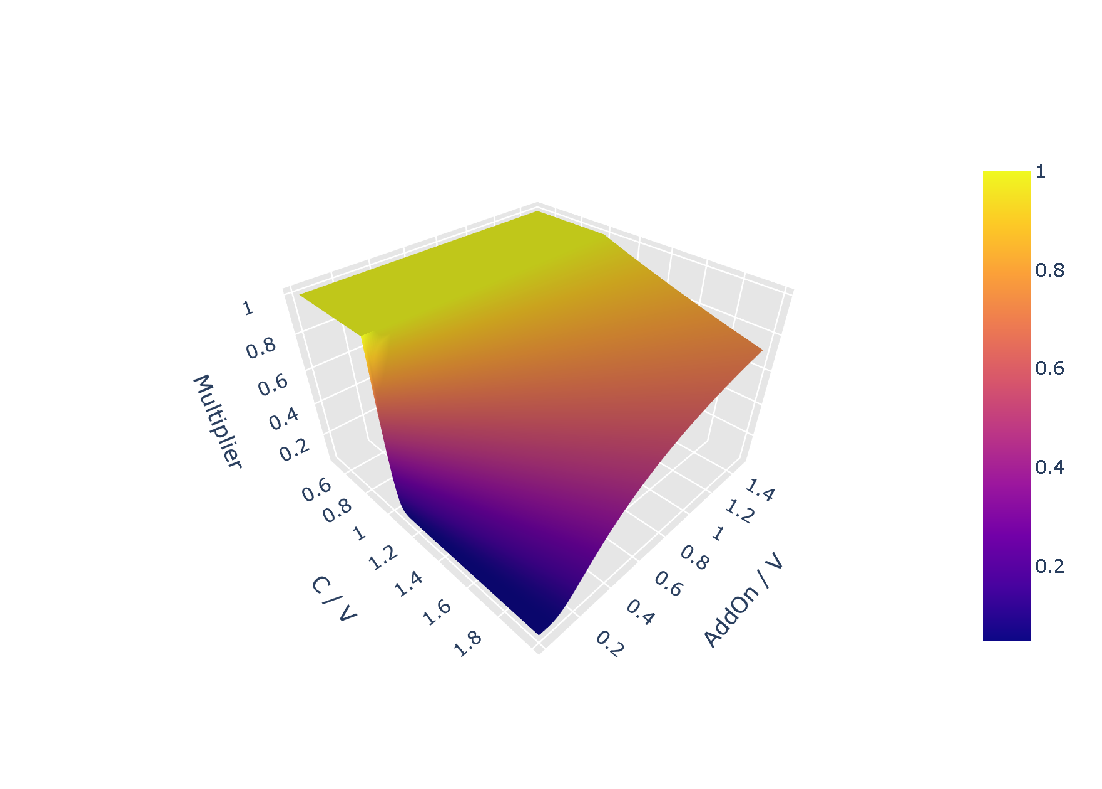
\includegraphics[scale=0.9]{Graphics/SACCR_Multiplier_Function.pdf}
	\caption{}
	\label{fig:multiplier}
\end{figure}

% \documentclass[11pt]{article}

    \usepackage[breakable]{tcolorbox}
    \usepackage{parskip} % Stop auto-indenting (to mimic markdown behaviour)
    
    \usepackage{iftex}
    \ifPDFTeX
    	\usepackage[T1]{fontenc}
    	\usepackage{mathpazo}
    \else
    	\usepackage{fontspec}
    \fi

    % Basic figure setup, for now with no caption control since it's done
    % automatically by Pandoc (which extracts ![](path) syntax from Markdown).
    \usepackage{graphicx}
    % Maintain compatibility with old templates. Remove in nbconvert 6.0
    \let\Oldincludegraphics\includegraphics
    % Ensure that by default, figures have no caption (until we provide a
    % proper Figure object with a Caption API and a way to capture that
    % in the conversion process - todo).
    \usepackage{caption}
    \DeclareCaptionFormat{nocaption}{}
    \captionsetup{format=nocaption,aboveskip=0pt,belowskip=0pt}

    \usepackage[Export]{adjustbox} % Used to constrain images to a maximum size
    \adjustboxset{max size={0.9\linewidth}{0.9\paperheight}}
    \usepackage{float}
    \floatplacement{figure}{H} % forces figures to be placed at the correct location
    \usepackage{xcolor} % Allow colors to be defined
    \usepackage{enumerate} % Needed for markdown enumerations to work
    \usepackage{geometry} % Used to adjust the document margins
    \usepackage{amsmath} % Equations
    \usepackage{amssymb} % Equations
    \usepackage{textcomp} % defines textquotesingle
    % Hack from http://tex.stackexchange.com/a/47451/13684:
    \AtBeginDocument{%
        \def\PYZsq{\textquotesingle}% Upright quotes in Pygmentized code
    }
    \usepackage{upquote} % Upright quotes for verbatim code
    \usepackage{eurosym} % defines \euro
    \usepackage[mathletters]{ucs} % Extended unicode (utf-8) support
    \usepackage{fancyvrb} % verbatim replacement that allows latex
    \usepackage{grffile} % extends the file name processing of package graphics 
                         % to support a larger range
    \makeatletter % fix for grffile with XeLaTeX
    \def\Gread@@xetex#1{%
      \IfFileExists{"\Gin@base".bb}%
      {\Gread@eps{\Gin@base.bb}}%
      {\Gread@@xetex@aux#1}%
    }
    \makeatother

    % The hyperref package gives us a pdf with properly built
    % internal navigation ('pdf bookmarks' for the table of contents,
    % internal cross-reference links, web links for URLs, etc.)
    \usepackage{hyperref}
    % The default LaTeX title has an obnoxious amount of whitespace. By default,
    % titling removes some of it. It also provides customization options.
    \usepackage{titling}
    \usepackage{longtable} % longtable support required by pandoc >1.10
    \usepackage{booktabs}  % table support for pandoc > 1.12.2
    \usepackage[inline]{enumitem} % IRkernel/repr support (it uses the enumerate* environment)
    \usepackage[normalem]{ulem} % ulem is needed to support strikethroughs (\sout)
                                % normalem makes italics be italics, not underlines
    \usepackage{mathrsfs}
    

    
    % Colors for the hyperref package
    \definecolor{urlcolor}{rgb}{0,.145,.698}
    \definecolor{linkcolor}{rgb}{.71,0.21,0.01}
    \definecolor{citecolor}{rgb}{.12,.54,.11}

    % ANSI colors
    \definecolor{ansi-black}{HTML}{3E424D}
    \definecolor{ansi-black-intense}{HTML}{282C36}
    \definecolor{ansi-red}{HTML}{E75C58}
    \definecolor{ansi-red-intense}{HTML}{B22B31}
    \definecolor{ansi-green}{HTML}{00A250}
    \definecolor{ansi-green-intense}{HTML}{007427}
    \definecolor{ansi-yellow}{HTML}{DDB62B}
    \definecolor{ansi-yellow-intense}{HTML}{B27D12}
    \definecolor{ansi-blue}{HTML}{208FFB}
    \definecolor{ansi-blue-intense}{HTML}{0065CA}
    \definecolor{ansi-magenta}{HTML}{D160C4}
    \definecolor{ansi-magenta-intense}{HTML}{A03196}
    \definecolor{ansi-cyan}{HTML}{60C6C8}
    \definecolor{ansi-cyan-intense}{HTML}{258F8F}
    \definecolor{ansi-white}{HTML}{C5C1B4}
    \definecolor{ansi-white-intense}{HTML}{A1A6B2}
    \definecolor{ansi-default-inverse-fg}{HTML}{FFFFFF}
    \definecolor{ansi-default-inverse-bg}{HTML}{000000}

    % commands and environments needed by pandoc snippets
    % extracted from the output of `pandoc -s`
    \providecommand{\tightlist}{%
      \setlength{\itemsep}{0pt}\setlength{\parskip}{0pt}}
    \DefineVerbatimEnvironment{Highlighting}{Verbatim}{commandchars=\\\{\}}
    % Add ',fontsize=\small' for more characters per line
    \newenvironment{Shaded}{}{}
    \newcommand{\KeywordTok}[1]{\textcolor[rgb]{0.00,0.44,0.13}{\textbf{{#1}}}}
    \newcommand{\DataTypeTok}[1]{\textcolor[rgb]{0.56,0.13,0.00}{{#1}}}
    \newcommand{\DecValTok}[1]{\textcolor[rgb]{0.25,0.63,0.44}{{#1}}}
    \newcommand{\BaseNTok}[1]{\textcolor[rgb]{0.25,0.63,0.44}{{#1}}}
    \newcommand{\FloatTok}[1]{\textcolor[rgb]{0.25,0.63,0.44}{{#1}}}
    \newcommand{\CharTok}[1]{\textcolor[rgb]{0.25,0.44,0.63}{{#1}}}
    \newcommand{\StringTok}[1]{\textcolor[rgb]{0.25,0.44,0.63}{{#1}}}
    \newcommand{\CommentTok}[1]{\textcolor[rgb]{0.38,0.63,0.69}{\textit{{#1}}}}
    \newcommand{\OtherTok}[1]{\textcolor[rgb]{0.00,0.44,0.13}{{#1}}}
    \newcommand{\AlertTok}[1]{\textcolor[rgb]{1.00,0.00,0.00}{\textbf{{#1}}}}
    \newcommand{\FunctionTok}[1]{\textcolor[rgb]{0.02,0.16,0.49}{{#1}}}
    \newcommand{\RegionMarkerTok}[1]{{#1}}
    \newcommand{\ErrorTok}[1]{\textcolor[rgb]{1.00,0.00,0.00}{\textbf{{#1}}}}
    \newcommand{\NormalTok}[1]{{#1}}
    
    % Additional commands for more recent versions of Pandoc
    \newcommand{\ConstantTok}[1]{\textcolor[rgb]{0.53,0.00,0.00}{{#1}}}
    \newcommand{\SpecialCharTok}[1]{\textcolor[rgb]{0.25,0.44,0.63}{{#1}}}
    \newcommand{\VerbatimStringTok}[1]{\textcolor[rgb]{0.25,0.44,0.63}{{#1}}}
    \newcommand{\SpecialStringTok}[1]{\textcolor[rgb]{0.73,0.40,0.53}{{#1}}}
    \newcommand{\ImportTok}[1]{{#1}}
    \newcommand{\DocumentationTok}[1]{\textcolor[rgb]{0.73,0.13,0.13}{\textit{{#1}}}}
    \newcommand{\AnnotationTok}[1]{\textcolor[rgb]{0.38,0.63,0.69}{\textbf{\textit{{#1}}}}}
    \newcommand{\CommentVarTok}[1]{\textcolor[rgb]{0.38,0.63,0.69}{\textbf{\textit{{#1}}}}}
    \newcommand{\VariableTok}[1]{\textcolor[rgb]{0.10,0.09,0.49}{{#1}}}
    \newcommand{\ControlFlowTok}[1]{\textcolor[rgb]{0.00,0.44,0.13}{\textbf{{#1}}}}
    \newcommand{\OperatorTok}[1]{\textcolor[rgb]{0.40,0.40,0.40}{{#1}}}
    \newcommand{\BuiltInTok}[1]{{#1}}
    \newcommand{\ExtensionTok}[1]{{#1}}
    \newcommand{\PreprocessorTok}[1]{\textcolor[rgb]{0.74,0.48,0.00}{{#1}}}
    \newcommand{\AttributeTok}[1]{\textcolor[rgb]{0.49,0.56,0.16}{{#1}}}
    \newcommand{\InformationTok}[1]{\textcolor[rgb]{0.38,0.63,0.69}{\textbf{\textit{{#1}}}}}
    \newcommand{\WarningTok}[1]{\textcolor[rgb]{0.38,0.63,0.69}{\textbf{\textit{{#1}}}}}
    
    
    % Define a nice break command that doesn't care if a line doesn't already
    % exist.
    \def\br{\hspace*{\fill} \\* }
    % Math Jax compatibility definitions
    \def\gt{>}
    \def\lt{<}
    \let\Oldtex\TeX
    \let\Oldlatex\LaTeX
    \renewcommand{\TeX}{\textrm{\Oldtex}}
    \renewcommand{\LaTeX}{\textrm{\Oldlatex}}
    % Document parameters
    % Document title
    \title{building\_SA\_CCR\_2}
    
    
    
    
    
% Pygments definitions
\makeatletter
\def\PY@reset{\let\PY@it=\relax \let\PY@bf=\relax%
    \let\PY@ul=\relax \let\PY@tc=\relax%
    \let\PY@bc=\relax \let\PY@ff=\relax}
\def\PY@tok#1{\csname PY@tok@#1\endcsname}
\def\PY@toks#1+{\ifx\relax#1\empty\else%
    \PY@tok{#1}\expandafter\PY@toks\fi}
\def\PY@do#1{\PY@bc{\PY@tc{\PY@ul{%
    \PY@it{\PY@bf{\PY@ff{#1}}}}}}}
\def\PY#1#2{\PY@reset\PY@toks#1+\relax+\PY@do{#2}}

\expandafter\def\csname PY@tok@w\endcsname{\def\PY@tc##1{\textcolor[rgb]{0.73,0.73,0.73}{##1}}}
\expandafter\def\csname PY@tok@c\endcsname{\let\PY@it=\textit\def\PY@tc##1{\textcolor[rgb]{0.25,0.50,0.50}{##1}}}
\expandafter\def\csname PY@tok@cp\endcsname{\def\PY@tc##1{\textcolor[rgb]{0.74,0.48,0.00}{##1}}}
\expandafter\def\csname PY@tok@k\endcsname{\let\PY@bf=\textbf\def\PY@tc##1{\textcolor[rgb]{0.00,0.50,0.00}{##1}}}
\expandafter\def\csname PY@tok@kp\endcsname{\def\PY@tc##1{\textcolor[rgb]{0.00,0.50,0.00}{##1}}}
\expandafter\def\csname PY@tok@kt\endcsname{\def\PY@tc##1{\textcolor[rgb]{0.69,0.00,0.25}{##1}}}
\expandafter\def\csname PY@tok@o\endcsname{\def\PY@tc##1{\textcolor[rgb]{0.40,0.40,0.40}{##1}}}
\expandafter\def\csname PY@tok@ow\endcsname{\let\PY@bf=\textbf\def\PY@tc##1{\textcolor[rgb]{0.67,0.13,1.00}{##1}}}
\expandafter\def\csname PY@tok@nb\endcsname{\def\PY@tc##1{\textcolor[rgb]{0.00,0.50,0.00}{##1}}}
\expandafter\def\csname PY@tok@nf\endcsname{\def\PY@tc##1{\textcolor[rgb]{0.00,0.00,1.00}{##1}}}
\expandafter\def\csname PY@tok@nc\endcsname{\let\PY@bf=\textbf\def\PY@tc##1{\textcolor[rgb]{0.00,0.00,1.00}{##1}}}
\expandafter\def\csname PY@tok@nn\endcsname{\let\PY@bf=\textbf\def\PY@tc##1{\textcolor[rgb]{0.00,0.00,1.00}{##1}}}
\expandafter\def\csname PY@tok@ne\endcsname{\let\PY@bf=\textbf\def\PY@tc##1{\textcolor[rgb]{0.82,0.25,0.23}{##1}}}
\expandafter\def\csname PY@tok@nv\endcsname{\def\PY@tc##1{\textcolor[rgb]{0.10,0.09,0.49}{##1}}}
\expandafter\def\csname PY@tok@no\endcsname{\def\PY@tc##1{\textcolor[rgb]{0.53,0.00,0.00}{##1}}}
\expandafter\def\csname PY@tok@nl\endcsname{\def\PY@tc##1{\textcolor[rgb]{0.63,0.63,0.00}{##1}}}
\expandafter\def\csname PY@tok@ni\endcsname{\let\PY@bf=\textbf\def\PY@tc##1{\textcolor[rgb]{0.60,0.60,0.60}{##1}}}
\expandafter\def\csname PY@tok@na\endcsname{\def\PY@tc##1{\textcolor[rgb]{0.49,0.56,0.16}{##1}}}
\expandafter\def\csname PY@tok@nt\endcsname{\let\PY@bf=\textbf\def\PY@tc##1{\textcolor[rgb]{0.00,0.50,0.00}{##1}}}
\expandafter\def\csname PY@tok@nd\endcsname{\def\PY@tc##1{\textcolor[rgb]{0.67,0.13,1.00}{##1}}}
\expandafter\def\csname PY@tok@s\endcsname{\def\PY@tc##1{\textcolor[rgb]{0.73,0.13,0.13}{##1}}}
\expandafter\def\csname PY@tok@sd\endcsname{\let\PY@it=\textit\def\PY@tc##1{\textcolor[rgb]{0.73,0.13,0.13}{##1}}}
\expandafter\def\csname PY@tok@si\endcsname{\let\PY@bf=\textbf\def\PY@tc##1{\textcolor[rgb]{0.73,0.40,0.53}{##1}}}
\expandafter\def\csname PY@tok@se\endcsname{\let\PY@bf=\textbf\def\PY@tc##1{\textcolor[rgb]{0.73,0.40,0.13}{##1}}}
\expandafter\def\csname PY@tok@sr\endcsname{\def\PY@tc##1{\textcolor[rgb]{0.73,0.40,0.53}{##1}}}
\expandafter\def\csname PY@tok@ss\endcsname{\def\PY@tc##1{\textcolor[rgb]{0.10,0.09,0.49}{##1}}}
\expandafter\def\csname PY@tok@sx\endcsname{\def\PY@tc##1{\textcolor[rgb]{0.00,0.50,0.00}{##1}}}
\expandafter\def\csname PY@tok@m\endcsname{\def\PY@tc##1{\textcolor[rgb]{0.40,0.40,0.40}{##1}}}
\expandafter\def\csname PY@tok@gh\endcsname{\let\PY@bf=\textbf\def\PY@tc##1{\textcolor[rgb]{0.00,0.00,0.50}{##1}}}
\expandafter\def\csname PY@tok@gu\endcsname{\let\PY@bf=\textbf\def\PY@tc##1{\textcolor[rgb]{0.50,0.00,0.50}{##1}}}
\expandafter\def\csname PY@tok@gd\endcsname{\def\PY@tc##1{\textcolor[rgb]{0.63,0.00,0.00}{##1}}}
\expandafter\def\csname PY@tok@gi\endcsname{\def\PY@tc##1{\textcolor[rgb]{0.00,0.63,0.00}{##1}}}
\expandafter\def\csname PY@tok@gr\endcsname{\def\PY@tc##1{\textcolor[rgb]{1.00,0.00,0.00}{##1}}}
\expandafter\def\csname PY@tok@ge\endcsname{\let\PY@it=\textit}
\expandafter\def\csname PY@tok@gs\endcsname{\let\PY@bf=\textbf}
\expandafter\def\csname PY@tok@gp\endcsname{\let\PY@bf=\textbf\def\PY@tc##1{\textcolor[rgb]{0.00,0.00,0.50}{##1}}}
\expandafter\def\csname PY@tok@go\endcsname{\def\PY@tc##1{\textcolor[rgb]{0.53,0.53,0.53}{##1}}}
\expandafter\def\csname PY@tok@gt\endcsname{\def\PY@tc##1{\textcolor[rgb]{0.00,0.27,0.87}{##1}}}
\expandafter\def\csname PY@tok@err\endcsname{\def\PY@bc##1{\setlength{\fboxsep}{0pt}\fcolorbox[rgb]{1.00,0.00,0.00}{1,1,1}{\strut ##1}}}
\expandafter\def\csname PY@tok@kc\endcsname{\let\PY@bf=\textbf\def\PY@tc##1{\textcolor[rgb]{0.00,0.50,0.00}{##1}}}
\expandafter\def\csname PY@tok@kd\endcsname{\let\PY@bf=\textbf\def\PY@tc##1{\textcolor[rgb]{0.00,0.50,0.00}{##1}}}
\expandafter\def\csname PY@tok@kn\endcsname{\let\PY@bf=\textbf\def\PY@tc##1{\textcolor[rgb]{0.00,0.50,0.00}{##1}}}
\expandafter\def\csname PY@tok@kr\endcsname{\let\PY@bf=\textbf\def\PY@tc##1{\textcolor[rgb]{0.00,0.50,0.00}{##1}}}
\expandafter\def\csname PY@tok@bp\endcsname{\def\PY@tc##1{\textcolor[rgb]{0.00,0.50,0.00}{##1}}}
\expandafter\def\csname PY@tok@fm\endcsname{\def\PY@tc##1{\textcolor[rgb]{0.00,0.00,1.00}{##1}}}
\expandafter\def\csname PY@tok@vc\endcsname{\def\PY@tc##1{\textcolor[rgb]{0.10,0.09,0.49}{##1}}}
\expandafter\def\csname PY@tok@vg\endcsname{\def\PY@tc##1{\textcolor[rgb]{0.10,0.09,0.49}{##1}}}
\expandafter\def\csname PY@tok@vi\endcsname{\def\PY@tc##1{\textcolor[rgb]{0.10,0.09,0.49}{##1}}}
\expandafter\def\csname PY@tok@vm\endcsname{\def\PY@tc##1{\textcolor[rgb]{0.10,0.09,0.49}{##1}}}
\expandafter\def\csname PY@tok@sa\endcsname{\def\PY@tc##1{\textcolor[rgb]{0.73,0.13,0.13}{##1}}}
\expandafter\def\csname PY@tok@sb\endcsname{\def\PY@tc##1{\textcolor[rgb]{0.73,0.13,0.13}{##1}}}
\expandafter\def\csname PY@tok@sc\endcsname{\def\PY@tc##1{\textcolor[rgb]{0.73,0.13,0.13}{##1}}}
\expandafter\def\csname PY@tok@dl\endcsname{\def\PY@tc##1{\textcolor[rgb]{0.73,0.13,0.13}{##1}}}
\expandafter\def\csname PY@tok@s2\endcsname{\def\PY@tc##1{\textcolor[rgb]{0.73,0.13,0.13}{##1}}}
\expandafter\def\csname PY@tok@sh\endcsname{\def\PY@tc##1{\textcolor[rgb]{0.73,0.13,0.13}{##1}}}
\expandafter\def\csname PY@tok@s1\endcsname{\def\PY@tc##1{\textcolor[rgb]{0.73,0.13,0.13}{##1}}}
\expandafter\def\csname PY@tok@mb\endcsname{\def\PY@tc##1{\textcolor[rgb]{0.40,0.40,0.40}{##1}}}
\expandafter\def\csname PY@tok@mf\endcsname{\def\PY@tc##1{\textcolor[rgb]{0.40,0.40,0.40}{##1}}}
\expandafter\def\csname PY@tok@mh\endcsname{\def\PY@tc##1{\textcolor[rgb]{0.40,0.40,0.40}{##1}}}
\expandafter\def\csname PY@tok@mi\endcsname{\def\PY@tc##1{\textcolor[rgb]{0.40,0.40,0.40}{##1}}}
\expandafter\def\csname PY@tok@il\endcsname{\def\PY@tc##1{\textcolor[rgb]{0.40,0.40,0.40}{##1}}}
\expandafter\def\csname PY@tok@mo\endcsname{\def\PY@tc##1{\textcolor[rgb]{0.40,0.40,0.40}{##1}}}
\expandafter\def\csname PY@tok@ch\endcsname{\let\PY@it=\textit\def\PY@tc##1{\textcolor[rgb]{0.25,0.50,0.50}{##1}}}
\expandafter\def\csname PY@tok@cm\endcsname{\let\PY@it=\textit\def\PY@tc##1{\textcolor[rgb]{0.25,0.50,0.50}{##1}}}
\expandafter\def\csname PY@tok@cpf\endcsname{\let\PY@it=\textit\def\PY@tc##1{\textcolor[rgb]{0.25,0.50,0.50}{##1}}}
\expandafter\def\csname PY@tok@c1\endcsname{\let\PY@it=\textit\def\PY@tc##1{\textcolor[rgb]{0.25,0.50,0.50}{##1}}}
\expandafter\def\csname PY@tok@cs\endcsname{\let\PY@it=\textit\def\PY@tc##1{\textcolor[rgb]{0.25,0.50,0.50}{##1}}}

\def\PYZbs{\char`\\}
\def\PYZus{\char`\_}
\def\PYZob{\char`\{}
\def\PYZcb{\char`\}}
\def\PYZca{\char`\^}
\def\PYZam{\char`\&}
\def\PYZlt{\char`\<}
\def\PYZgt{\char`\>}
\def\PYZsh{\char`\#}
\def\PYZpc{\char`\%}
\def\PYZdl{\char`\$}
\def\PYZhy{\char`\-}
\def\PYZsq{\char`\'}
\def\PYZdq{\char`\"}
\def\PYZti{\char`\~}
% for compatibility with earlier versions
\def\PYZat{@}
\def\PYZlb{[}
\def\PYZrb{]}
\makeatother


    % For linebreaks inside Verbatim environment from package fancyvrb. 
    \makeatletter
        \newbox\Wrappedcontinuationbox 
        \newbox\Wrappedvisiblespacebox 
        \newcommand*\Wrappedvisiblespace {\textcolor{red}{\textvisiblespace}} 
        \newcommand*\Wrappedcontinuationsymbol {\textcolor{red}{\llap{\tiny$\m@th\hookrightarrow$}}} 
        \newcommand*\Wrappedcontinuationindent {3ex } 
        \newcommand*\Wrappedafterbreak {\kern\Wrappedcontinuationindent\copy\Wrappedcontinuationbox} 
        % Take advantage of the already applied Pygments mark-up to insert 
        % potential linebreaks for TeX processing. 
        %        {, <, #, %, $, ' and ": go to next line. 
        %        _, }, ^, &, >, - and ~: stay at end of broken line. 
        % Use of \textquotesingle for straight quote. 
        \newcommand*\Wrappedbreaksatspecials {% 
            \def\PYGZus{\discretionary{\char`\_}{\Wrappedafterbreak}{\char`\_}}% 
            \def\PYGZob{\discretionary{}{\Wrappedafterbreak\char`\{}{\char`\{}}% 
            \def\PYGZcb{\discretionary{\char`\}}{\Wrappedafterbreak}{\char`\}}}% 
            \def\PYGZca{\discretionary{\char`\^}{\Wrappedafterbreak}{\char`\^}}% 
            \def\PYGZam{\discretionary{\char`\&}{\Wrappedafterbreak}{\char`\&}}% 
            \def\PYGZlt{\discretionary{}{\Wrappedafterbreak\char`\<}{\char`\<}}% 
            \def\PYGZgt{\discretionary{\char`\>}{\Wrappedafterbreak}{\char`\>}}% 
            \def\PYGZsh{\discretionary{}{\Wrappedafterbreak\char`\#}{\char`\#}}% 
            \def\PYGZpc{\discretionary{}{\Wrappedafterbreak\char`\%}{\char`\%}}% 
            \def\PYGZdl{\discretionary{}{\Wrappedafterbreak\char`\$}{\char`\$}}% 
            \def\PYGZhy{\discretionary{\char`\-}{\Wrappedafterbreak}{\char`\-}}% 
            \def\PYGZsq{\discretionary{}{\Wrappedafterbreak\textquotesingle}{\textquotesingle}}% 
            \def\PYGZdq{\discretionary{}{\Wrappedafterbreak\char`\"}{\char`\"}}% 
            \def\PYGZti{\discretionary{\char`\~}{\Wrappedafterbreak}{\char`\~}}% 
        } 
        % Some characters . , ; ? ! / are not pygmentized. 
        % This macro makes them "active" and they will insert potential linebreaks 
        \newcommand*\Wrappedbreaksatpunct {% 
            \lccode`\~`\.\lowercase{\def~}{\discretionary{\hbox{\char`\.}}{\Wrappedafterbreak}{\hbox{\char`\.}}}% 
            \lccode`\~`\,\lowercase{\def~}{\discretionary{\hbox{\char`\,}}{\Wrappedafterbreak}{\hbox{\char`\,}}}% 
            \lccode`\~`\;\lowercase{\def~}{\discretionary{\hbox{\char`\;}}{\Wrappedafterbreak}{\hbox{\char`\;}}}% 
            \lccode`\~`\:\lowercase{\def~}{\discretionary{\hbox{\char`\:}}{\Wrappedafterbreak}{\hbox{\char`\:}}}% 
            \lccode`\~`\?\lowercase{\def~}{\discretionary{\hbox{\char`\?}}{\Wrappedafterbreak}{\hbox{\char`\?}}}% 
            \lccode`\~`\!\lowercase{\def~}{\discretionary{\hbox{\char`\!}}{\Wrappedafterbreak}{\hbox{\char`\!}}}% 
            \lccode`\~`\/\lowercase{\def~}{\discretionary{\hbox{\char`\/}}{\Wrappedafterbreak}{\hbox{\char`\/}}}% 
            \catcode`\.\active
            \catcode`\,\active 
            \catcode`\;\active
            \catcode`\:\active
            \catcode`\?\active
            \catcode`\!\active
            \catcode`\/\active 
            \lccode`\~`\~ 	
        }
    \makeatother

    \let\OriginalVerbatim=\Verbatim
    \makeatletter
    \renewcommand{\Verbatim}[1][1]{%
        %\parskip\z@skip
        \sbox\Wrappedcontinuationbox {\Wrappedcontinuationsymbol}%
        \sbox\Wrappedvisiblespacebox {\FV@SetupFont\Wrappedvisiblespace}%
        \def\FancyVerbFormatLine ##1{\hsize\linewidth
            \vtop{\raggedright\hyphenpenalty\z@\exhyphenpenalty\z@
                \doublehyphendemerits\z@\finalhyphendemerits\z@
                \strut ##1\strut}%
        }%
        % If the linebreak is at a space, the latter will be displayed as visible
        % space at end of first line, and a continuation symbol starts next line.
        % Stretch/shrink are however usually zero for typewriter font.
        \def\FV@Space {%
            \nobreak\hskip\z@ plus\fontdimen3\font minus\fontdimen4\font
            \discretionary{\copy\Wrappedvisiblespacebox}{\Wrappedafterbreak}
            {\kern\fontdimen2\font}%
        }%
        
        % Allow breaks at special characters using \PYG... macros.
        \Wrappedbreaksatspecials
        % Breaks at punctuation characters . , ; ? ! and / need catcode=\active 	
        \OriginalVerbatim[#1,codes*=\Wrappedbreaksatpunct]%
    }
    \makeatother

    % Exact colors from NB
    \definecolor{incolor}{HTML}{303F9F}
    \definecolor{outcolor}{HTML}{D84315}
    \definecolor{cellborder}{HTML}{CFCFCF}
    \definecolor{cellbackground}{HTML}{F7F7F7}
    
    % prompt
    \makeatletter
    \newcommand{\boxspacing}{\kern\kvtcb@left@rule\kern\kvtcb@boxsep}
    \makeatother
    \newcommand{\prompt}[4]{
        \ttfamily\llap{{\color{#2}[#3]:\hspace{3pt}#4}}\vspace{-\baselineskip}
    }
    

    
    % Prevent overflowing lines due to hard-to-break entities
    \sloppy 
    % Setup hyperref package
    \hypersetup{
      breaklinks=true,  % so long urls are correctly broken across lines
      colorlinks=true,
      urlcolor=urlcolor,
      linkcolor=linkcolor,
      citecolor=citecolor,
      }
    % Slightly bigger margins than the latex defaults
    
    \geometry{verbose,tmargin=1in,bmargin=1in,lmargin=1in,rmargin=1in}
    
    

\begin{document}
    
    \maketitle
    
    

    
    \hypertarget{addon-calculation}{%
\subsubsection{AddOn calculation}\label{addon-calculation}}

Most of the SA-CCR logic is hidden inside the AddOn calculation. At
first it is important to define the following four data parameters:

\hypertarget{m_i}{%
\subparagraph{\texorpdfstring{\(M_i\)}{M\_i}}\label{m_i}}

\begin{quote}
Maturity of the derivative contract. If the underlying of a derivative
is another derivative - e.g.~in the case of a swaption the maturity date
of the underlying needs to be chosen.
\end{quote}

\hypertarget{s_i}{%
\subparagraph{\texorpdfstring{\(S_i\)}{S\_i}}\label{s_i}}

\begin{quote}
For interest rate and credit derivatives the start date of the time
periodreferenced by an interst rate or credit contract. If the
derivtives underlying is another interest rate or credit intsrument (eg
swaption or bond option) \(S_i\) is the start date of the underlying
instead.
\end{quote}

\hypertarget{e_i}{%
\subparagraph{\texorpdfstring{\(E_i\)}{E\_i}}\label{e_i}}

\begin{quote}
Defined as \(S_i\) but referencing the end date instead of the start
date.
\end{quote}

\hypertarget{t_i}{%
\subparagraph{\texorpdfstring{\(T_i\)}{T\_i}}\label{t_i}}

\begin{quote}
For options across all asset classes this is the latest contractual
exercise date.
\end{quote}

    \hypertarget{trade-level-adjusted-notional}{%
\subsection{Trade level adjusted
notional}\label{trade-level-adjusted-notional}}

Each trade \(i\) has a trade level adjusted notional \(d_i^a\) assigned
to it. This is calculated differently for the different asset classes.

\hypertarget{interest-rate-and-credit-derivatives}{%
\paragraph{Interest rate and credit
derivatives}\label{interest-rate-and-credit-derivatives}}

\begin{quote}
The notional of the trade is usually a well defined value in domestic
currency for interest rate and credit derivatives. It is multiplied by a
supervisory duration factor. The basic idea is, that the value of the
derivative can change more the longer the remaining
\end{quote}

\begin{align*}
d_i &= \text{Notional}_i * SD_i \\
\\
\text{where} \qquad SD_i &=\frac{\exp\left(-0.05 * S_i\right)-\exp\left(-0.05 * E_i\right)}{0.05}
\end{align*}

\hypertarget{fx-derivatives}{%
\paragraph{FX derivatives}\label{fx-derivatives}}

\begin{quote}
While the wording in the BCBS paper is a bit more specific we will just
assume that every FX traded derivative has a USD leg and set the
notional equal the to USD notional.
\end{quote}

\hypertarget{equity-and-commodity-derivatives}{%
\paragraph{Equity and commodity
derivatives}\label{equity-and-commodity-derivatives}}

\begin{quote}
The notional is defined as the price of the underlying. Therefore, it
fluctuates over time.
\end{quote}

\hypertarget{notional-of-exotic-derivatives}{%
\paragraph{Notional of exotic
derivatives}\label{notional-of-exotic-derivatives}}

\begin{quote}
For more exotic derivatives which do have adjustable notionals,
resetting notionals etc. detailed handling of the notional is defined in
paragraph 158.
\end{quote}

    Within this thesis we investigate only equity and interest rate
derivatives. For these we can make a few exemplary calculations of the
trade level adjusted notional.

For equity trades determining the trade level adjusted notional is
trivial as it always is the spot price of the underlying. As an example
consider the two trades defined below:

    \begin{tcolorbox}[breakable, size=fbox, boxrule=1pt, pad at break*=1mm,colback=cellbackground, colframe=cellborder]
\prompt{In}{incolor}{2}{\boxspacing}
\begin{Verbatim}[commandchars=\\\{\}]
\PY{c+c1}{\PYZsh{}When the strike is not set explicitly an at the money option is created with K = S(t0)}
\PY{n}{eqOption1} \PY{o}{=} \PY{n}{EquityOption}\PY{p}{(}\PY{n}{maturity} \PY{o}{=} \PY{n}{ql}\PY{o}{.}\PY{n}{Period}\PY{p}{(}\PY{l+m+mi}{1}\PY{p}{,} \PY{n}{ql}\PY{o}{.}\PY{n}{Years}\PY{p}{)}\PY{p}{,}
                         \PY{n}{tradeType}\PY{o}{=} \PY{n}{TradeType}\PY{o}{.}\PY{n}{CALL}\PY{p}{,}
                         \PY{n}{tradeDirection}\PY{o}{=} \PY{n}{TradeDirection}\PY{o}{.}\PY{n}{LONG}\PY{p}{,}
                         \PY{n}{underlying}\PY{o}{=} \PY{n}{Stock}\PY{o}{.}\PY{n}{ADS}\PY{p}{)}

\PY{n}{eqOption2} \PY{o}{=} \PY{n}{EquityOption}\PY{p}{(}\PY{n}{maturity} \PY{o}{=} \PY{n}{ql}\PY{o}{.}\PY{n}{Period}\PY{p}{(}\PY{l+m+mi}{1}\PY{p}{,}   \PY{n}{ql}\PY{o}{.}\PY{n}{Years}\PY{p}{)}\PY{p}{,}
                         \PY{n}{tradeType}\PY{o}{=} \PY{n}{TradeType}\PY{o}{.}\PY{n}{PUT}\PY{p}{,}
                         \PY{n}{tradeDirection}\PY{o}{=} \PY{n}{TradeDirection}\PY{o}{.}\PY{n}{SHORT}\PY{p}{,}
                         \PY{n}{underlying}\PY{o}{=} \PY{n}{Stock}\PY{o}{.}\PY{n}{ADS}\PY{p}{,}
                         \PY{n}{strike} \PY{o}{=} \PY{l+m+mi}{60}\PY{p}{)}
\end{Verbatim}
\end{tcolorbox}

    Let the spot price of Adidas stock be 42. Then, the adjusted notional of
\texttt{eqOption1}, an at the money call on Adidas, is 42 and the
adjusted notional of \texttt{eqOption2}, a short in the money put on
Adidas, is also 42.

    
    For interest rate derivatives such as interest rate swaps or swaptions
on the other hand, the notional is adjusted by the supervisory duration
factor. As the supervisory duration depends on \emph{S} and \emph{E} it
is important to understand how these are determined for the different
interest rate derivatives.

\begin{longtable}[]{@{}lll@{}}
\toprule
\begin{minipage}[b]{0.24\columnwidth}\raggedright
Trade Type\strut
\end{minipage} & \begin{minipage}[b]{0.32\columnwidth}\raggedright
\emph{S}\strut
\end{minipage} & \begin{minipage}[b]{0.36\columnwidth}\raggedright
\emph{E}\strut
\end{minipage}\tabularnewline
\midrule
\endhead
\begin{minipage}[t]{0.24\columnwidth}\raggedright
\textbf{Interest Rate Swap}\strut
\end{minipage} & \begin{minipage}[t]{0.32\columnwidth}\raggedright
Current date\strut
\end{minipage} & \begin{minipage}[t]{0.36\columnwidth}\raggedright
Maturity date\strut
\end{minipage}\tabularnewline
\begin{minipage}[t]{0.24\columnwidth}\raggedright
\textbf{Forward starting IRS}\strut
\end{minipage} & \begin{minipage}[t]{0.32\columnwidth}\raggedright
Start date of the underlying swap\strut
\end{minipage} & \begin{minipage}[t]{0.36\columnwidth}\raggedright
Maturity date of the underlying swap\strut
\end{minipage}\tabularnewline
\begin{minipage}[t]{0.24\columnwidth}\raggedright
\textbf{Swaption}\strut
\end{minipage} & \begin{minipage}[t]{0.32\columnwidth}\raggedright
Start date of the underlying swap\strut
\end{minipage} & \begin{minipage}[t]{0.36\columnwidth}\raggedright
Maturity data of the underlying swap\strut
\end{minipage}\tabularnewline
\bottomrule
\end{longtable}

    \hypertarget{supervisory-delta-adjustments}{%
\subsection{Supervisory delta
adjustments}\label{supervisory-delta-adjustments}}

For linear derivatives \(\delta\) is 1 for long derivatives and -1 for
short derivatives.

For options \(\delta\) is defined as under Black-Scholes:

\begin{align*}
\delta_{\text{long Call}} &= +\Phi\left(\frac{\ln\left(P_i / K_i \right) + 0.5 * \sigma_i^2 * T_i}{\sigma_i * \sqrt{T_i}}\right) \\
\\
\text{where} \qquad \Phi &: \text{standard normal cdf} \\
\sigma_i &: \text{supervisory volatility as defined in Table 2 in paragraph 183}
\end{align*}

This delta is multiplied by -1 in case of a long Put option or a short
Call option. This formula is used for both, equity options and
swaptions.

No detail is given at this point on the delta calculation of CDO
tranches as these are not in the scope of this thesis.

    In the case of an european equity option the parametrization is quite
straight forward.

\(\sigma_i\): 1.2 is the supervisory volatility for a single stock
option

\(K_i\): The strike of the option

\(P_i\): The spot price of the underlying stock

\(T_i\): The maturity of the option

A swaption on the other hand is parametrized as follows for calculation
of its supervisory delta:

\(\sigma_i\): 0.5 is the supervisory volatility for any interst rate
option.

\(K_i\): The strike of the option is the fixed rate of the underlying
swap

\(P_i\): Is the current par rate of the underlying (forward starting)
swap

\(T_i\): The maturity of the option. Please note the difference to
\(E_i\) used for calculation of the adjusted notional, which is the
maturity of the underlying swap.

SA-CCR uses the same Black-Scholes based formula for Swaps as it uses
for Equities. It differentiates options in two dimensions. Whether they
are \emph{bought} or \emph{sold} and whether they are \emph{Call} or
\emph{Put} options (Compare paragraph 159).

SA-CCR defines an option as a call option if it rises in value as the
underlying rises in value. A fixed payer swap rises in value as the
underlying interest rate rises in value. Therefore, an option to buy a
fixed payer swap at a predetermined strike also rises in value as the
underlying interest rate rises in value. Therefore, a swaption on a
payer swap is considered a \emph{Call} under SA-CCR, while a swaption on
a receiver swap is considered a \emph{Put}.

    For the at the money option \texttt{eqOption1} that was set up above we
yield a supervisory delta adjustment of 0.7257.

    
    For an examplary short european swaption that has a par swap as
underlying (i.e.~the NPV of the swap is 0) that is set up as follows:

    \begin{tcolorbox}[breakable, size=fbox, boxrule=1pt, pad at break*=1mm,colback=cellbackground, colframe=cellborder]
\prompt{In}{incolor}{9}{\boxspacing}
\begin{Verbatim}[commandchars=\\\{\}]
\PY{n}{swap} \PY{o}{=} \PY{n}{IRS}\PY{p}{(}\PY{n}{notional}\PY{o}{=}\PY{l+m+mi}{100}\PY{p}{,}
           \PY{n}{timeToSwapStart}\PY{o}{=}\PY{n}{ql}\PY{o}{.}\PY{n}{Period}\PY{p}{(}\PY{l+m+mi}{1}\PY{p}{,} \PY{n}{ql}\PY{o}{.}\PY{n}{Years}\PY{p}{)}\PY{p}{,}
           \PY{n}{timeToSwapEnd}\PY{o}{=}\PY{n}{ql}\PY{o}{.}\PY{n}{Period}\PY{p}{(}\PY{l+m+mi}{3}\PY{p}{,} \PY{n}{ql}\PY{o}{.}\PY{n}{Years}\PY{p}{)}\PY{p}{,}
           \PY{n}{swapDirection}\PY{o}{=}\PY{n}{SwapDirection}\PY{o}{.}\PY{n}{PAYER}\PY{p}{,}
           \PY{n}{index}\PY{o}{=}\PY{n}{InterestRateIndex}\PY{o}{.}\PY{n}{EURIBOR6M}
          \PY{p}{)}

\PY{n}{swaption} \PY{o}{=} \PY{n}{Swaption}\PY{p}{(}\PY{n}{underlyingSwap}\PY{o}{=}\PY{n}{swap}\PY{p}{,}
                    \PY{n}{optionMaturity}\PY{o}{=}\PY{n}{ql}\PY{o}{.}\PY{n}{Period}\PY{p}{(}\PY{l+m+mi}{1}\PY{p}{,} \PY{n}{ql}\PY{o}{.}\PY{n}{Years}\PY{p}{)}\PY{p}{,}
                    \PY{n}{tradeDirection}\PY{o}{=}\PY{n}{TradeDirection}\PY{o}{.}\PY{n}{SHORT}\PY{p}{)}

\PY{n}{SA\PYZus{}CCR}\PY{o}{.}\PY{n}{calculate\PYZus{}sa\PYZus{}ccr\PYZus{}delta}\PY{p}{(}\PY{n}{swaption}\PY{p}{)}
\end{Verbatim}
\end{tcolorbox}

            \begin{tcolorbox}[breakable, size=fbox, boxrule=.5pt, pad at break*=1mm, opacityfill=0]
\prompt{Out}{outcolor}{9}{\boxspacing}
\begin{Verbatim}[commandchars=\\\{\}]
-0.5987063256829928
\end{Verbatim}
\end{tcolorbox}
        
    we yield a regulatory delta of -0.5987.

    

    % Add a bibliography block to the postdoc
    
    
    
\end{document}


%     

    
    However, the approach of SA-CCR to use the Black-Scholes for interest
rate derivatives does have a significant flaw.

Obviously, \(\ln\left(P_i / K_i \right)\) is not defined, if \(P_i/K_i\)
is negative. This has, however been very commonplace in recent years,
especially for Euro swaptions. One can always set the fixed rate of the
underlying swap and therefore \(K_i\) as a negative value. But based on
the market data of the 10th of May 2019 it is even possible to yield
negative par rates for the underlying swap.

As an example we are plotting the zero and the 6M forward curve for the
EURIBOR 6M index below. When zooming further in, we can see that that
the 6M forward curve crosses 0 on the 15th of November 2021.




% \begin{figure}
% 	\centering
% 	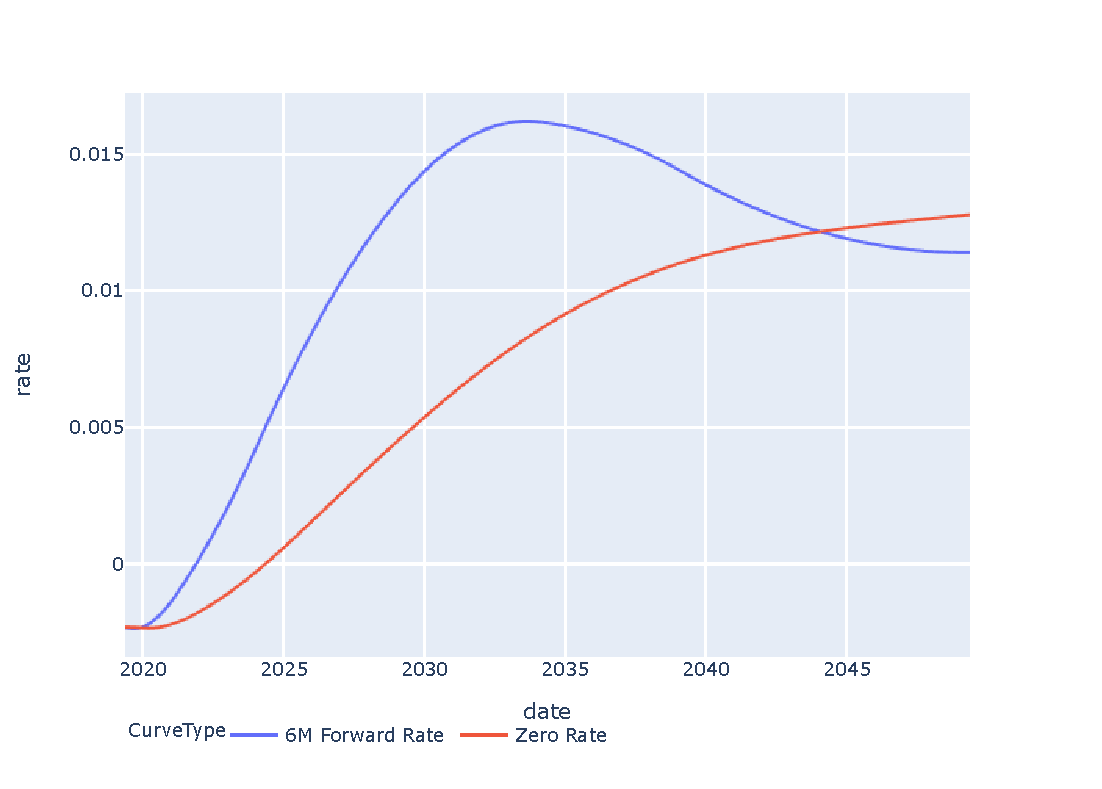
\includegraphics[scale=0.95]{../Graphics/euribor6m_termstructure.pdf}
%     \caption{}
% \end{figure}

% \begin{figure}
% 	\centering
% 	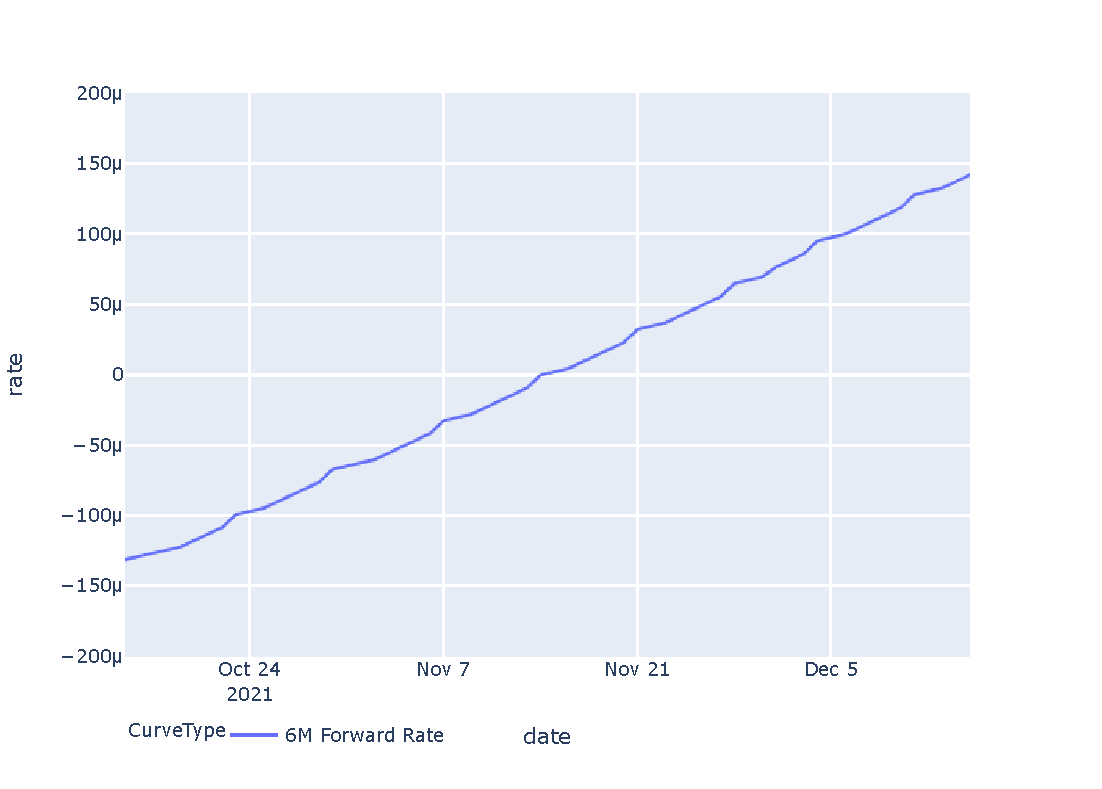
\includegraphics[scale=0.95]{../Graphics/euribor6m_termstructure_crossing_zero.pdf}
%     \caption{}
% \end{figure}

% \documentclass[11pt]{article}

    \usepackage[breakable]{tcolorbox}
    \usepackage{parskip} % Stop auto-indenting (to mimic markdown behaviour)
    
    \usepackage{iftex}
    \ifPDFTeX
    	\usepackage[T1]{fontenc}
    	\usepackage{mathpazo}
    \else
    	\usepackage{fontspec}
    \fi

    % Basic figure setup, for now with no caption control since it's done
    % automatically by Pandoc (which extracts ![](path) syntax from Markdown).
    \usepackage{graphicx}
    % Maintain compatibility with old templates. Remove in nbconvert 6.0
    \let\Oldincludegraphics\includegraphics
    % Ensure that by default, figures have no caption (until we provide a
    % proper Figure object with a Caption API and a way to capture that
    % in the conversion process - todo).
    \usepackage{caption}
    \DeclareCaptionFormat{nocaption}{}
    \captionsetup{format=nocaption,aboveskip=0pt,belowskip=0pt}

    \usepackage[Export]{adjustbox} % Used to constrain images to a maximum size
    \adjustboxset{max size={0.9\linewidth}{0.9\paperheight}}
    \usepackage{float}
    \floatplacement{figure}{H} % forces figures to be placed at the correct location
    \usepackage{xcolor} % Allow colors to be defined
    \usepackage{enumerate} % Needed for markdown enumerations to work
    \usepackage{geometry} % Used to adjust the document margins
    \usepackage{amsmath} % Equations
    \usepackage{amssymb} % Equations
    \usepackage{textcomp} % defines textquotesingle
    % Hack from http://tex.stackexchange.com/a/47451/13684:
    \AtBeginDocument{%
        \def\PYZsq{\textquotesingle}% Upright quotes in Pygmentized code
    }
    \usepackage{upquote} % Upright quotes for verbatim code
    \usepackage{eurosym} % defines \euro
    \usepackage[mathletters]{ucs} % Extended unicode (utf-8) support
    \usepackage{fancyvrb} % verbatim replacement that allows latex
    \usepackage{grffile} % extends the file name processing of package graphics 
                         % to support a larger range
    \makeatletter % fix for grffile with XeLaTeX
    \def\Gread@@xetex#1{%
      \IfFileExists{"\Gin@base".bb}%
      {\Gread@eps{\Gin@base.bb}}%
      {\Gread@@xetex@aux#1}%
    }
    \makeatother

    % The hyperref package gives us a pdf with properly built
    % internal navigation ('pdf bookmarks' for the table of contents,
    % internal cross-reference links, web links for URLs, etc.)
    \usepackage{hyperref}
    % The default LaTeX title has an obnoxious amount of whitespace. By default,
    % titling removes some of it. It also provides customization options.
    \usepackage{titling}
    \usepackage{longtable} % longtable support required by pandoc >1.10
    \usepackage{booktabs}  % table support for pandoc > 1.12.2
    \usepackage[inline]{enumitem} % IRkernel/repr support (it uses the enumerate* environment)
    \usepackage[normalem]{ulem} % ulem is needed to support strikethroughs (\sout)
                                % normalem makes italics be italics, not underlines
    \usepackage{mathrsfs}
    

    
    % Colors for the hyperref package
    \definecolor{urlcolor}{rgb}{0,.145,.698}
    \definecolor{linkcolor}{rgb}{.71,0.21,0.01}
    \definecolor{citecolor}{rgb}{.12,.54,.11}

    % ANSI colors
    \definecolor{ansi-black}{HTML}{3E424D}
    \definecolor{ansi-black-intense}{HTML}{282C36}
    \definecolor{ansi-red}{HTML}{E75C58}
    \definecolor{ansi-red-intense}{HTML}{B22B31}
    \definecolor{ansi-green}{HTML}{00A250}
    \definecolor{ansi-green-intense}{HTML}{007427}
    \definecolor{ansi-yellow}{HTML}{DDB62B}
    \definecolor{ansi-yellow-intense}{HTML}{B27D12}
    \definecolor{ansi-blue}{HTML}{208FFB}
    \definecolor{ansi-blue-intense}{HTML}{0065CA}
    \definecolor{ansi-magenta}{HTML}{D160C4}
    \definecolor{ansi-magenta-intense}{HTML}{A03196}
    \definecolor{ansi-cyan}{HTML}{60C6C8}
    \definecolor{ansi-cyan-intense}{HTML}{258F8F}
    \definecolor{ansi-white}{HTML}{C5C1B4}
    \definecolor{ansi-white-intense}{HTML}{A1A6B2}
    \definecolor{ansi-default-inverse-fg}{HTML}{FFFFFF}
    \definecolor{ansi-default-inverse-bg}{HTML}{000000}

    % commands and environments needed by pandoc snippets
    % extracted from the output of `pandoc -s`
    \providecommand{\tightlist}{%
      \setlength{\itemsep}{0pt}\setlength{\parskip}{0pt}}
    \DefineVerbatimEnvironment{Highlighting}{Verbatim}{commandchars=\\\{\}}
    % Add ',fontsize=\small' for more characters per line
    \newenvironment{Shaded}{}{}
    \newcommand{\KeywordTok}[1]{\textcolor[rgb]{0.00,0.44,0.13}{\textbf{{#1}}}}
    \newcommand{\DataTypeTok}[1]{\textcolor[rgb]{0.56,0.13,0.00}{{#1}}}
    \newcommand{\DecValTok}[1]{\textcolor[rgb]{0.25,0.63,0.44}{{#1}}}
    \newcommand{\BaseNTok}[1]{\textcolor[rgb]{0.25,0.63,0.44}{{#1}}}
    \newcommand{\FloatTok}[1]{\textcolor[rgb]{0.25,0.63,0.44}{{#1}}}
    \newcommand{\CharTok}[1]{\textcolor[rgb]{0.25,0.44,0.63}{{#1}}}
    \newcommand{\StringTok}[1]{\textcolor[rgb]{0.25,0.44,0.63}{{#1}}}
    \newcommand{\CommentTok}[1]{\textcolor[rgb]{0.38,0.63,0.69}{\textit{{#1}}}}
    \newcommand{\OtherTok}[1]{\textcolor[rgb]{0.00,0.44,0.13}{{#1}}}
    \newcommand{\AlertTok}[1]{\textcolor[rgb]{1.00,0.00,0.00}{\textbf{{#1}}}}
    \newcommand{\FunctionTok}[1]{\textcolor[rgb]{0.02,0.16,0.49}{{#1}}}
    \newcommand{\RegionMarkerTok}[1]{{#1}}
    \newcommand{\ErrorTok}[1]{\textcolor[rgb]{1.00,0.00,0.00}{\textbf{{#1}}}}
    \newcommand{\NormalTok}[1]{{#1}}
    
    % Additional commands for more recent versions of Pandoc
    \newcommand{\ConstantTok}[1]{\textcolor[rgb]{0.53,0.00,0.00}{{#1}}}
    \newcommand{\SpecialCharTok}[1]{\textcolor[rgb]{0.25,0.44,0.63}{{#1}}}
    \newcommand{\VerbatimStringTok}[1]{\textcolor[rgb]{0.25,0.44,0.63}{{#1}}}
    \newcommand{\SpecialStringTok}[1]{\textcolor[rgb]{0.73,0.40,0.53}{{#1}}}
    \newcommand{\ImportTok}[1]{{#1}}
    \newcommand{\DocumentationTok}[1]{\textcolor[rgb]{0.73,0.13,0.13}{\textit{{#1}}}}
    \newcommand{\AnnotationTok}[1]{\textcolor[rgb]{0.38,0.63,0.69}{\textbf{\textit{{#1}}}}}
    \newcommand{\CommentVarTok}[1]{\textcolor[rgb]{0.38,0.63,0.69}{\textbf{\textit{{#1}}}}}
    \newcommand{\VariableTok}[1]{\textcolor[rgb]{0.10,0.09,0.49}{{#1}}}
    \newcommand{\ControlFlowTok}[1]{\textcolor[rgb]{0.00,0.44,0.13}{\textbf{{#1}}}}
    \newcommand{\OperatorTok}[1]{\textcolor[rgb]{0.40,0.40,0.40}{{#1}}}
    \newcommand{\BuiltInTok}[1]{{#1}}
    \newcommand{\ExtensionTok}[1]{{#1}}
    \newcommand{\PreprocessorTok}[1]{\textcolor[rgb]{0.74,0.48,0.00}{{#1}}}
    \newcommand{\AttributeTok}[1]{\textcolor[rgb]{0.49,0.56,0.16}{{#1}}}
    \newcommand{\InformationTok}[1]{\textcolor[rgb]{0.38,0.63,0.69}{\textbf{\textit{{#1}}}}}
    \newcommand{\WarningTok}[1]{\textcolor[rgb]{0.38,0.63,0.69}{\textbf{\textit{{#1}}}}}
    
    
    % Define a nice break command that doesn't care if a line doesn't already
    % exist.
    \def\br{\hspace*{\fill} \\* }
    % Math Jax compatibility definitions
    \def\gt{>}
    \def\lt{<}
    \let\Oldtex\TeX
    \let\Oldlatex\LaTeX
    \renewcommand{\TeX}{\textrm{\Oldtex}}
    \renewcommand{\LaTeX}{\textrm{\Oldlatex}}
    % Document parameters
    % Document title
    \title{issue\_regulatory\_swaption\_delta\_2}
    
    
    
    
    
% Pygments definitions
\makeatletter
\def\PY@reset{\let\PY@it=\relax \let\PY@bf=\relax%
    \let\PY@ul=\relax \let\PY@tc=\relax%
    \let\PY@bc=\relax \let\PY@ff=\relax}
\def\PY@tok#1{\csname PY@tok@#1\endcsname}
\def\PY@toks#1+{\ifx\relax#1\empty\else%
    \PY@tok{#1}\expandafter\PY@toks\fi}
\def\PY@do#1{\PY@bc{\PY@tc{\PY@ul{%
    \PY@it{\PY@bf{\PY@ff{#1}}}}}}}
\def\PY#1#2{\PY@reset\PY@toks#1+\relax+\PY@do{#2}}

\expandafter\def\csname PY@tok@w\endcsname{\def\PY@tc##1{\textcolor[rgb]{0.73,0.73,0.73}{##1}}}
\expandafter\def\csname PY@tok@c\endcsname{\let\PY@it=\textit\def\PY@tc##1{\textcolor[rgb]{0.25,0.50,0.50}{##1}}}
\expandafter\def\csname PY@tok@cp\endcsname{\def\PY@tc##1{\textcolor[rgb]{0.74,0.48,0.00}{##1}}}
\expandafter\def\csname PY@tok@k\endcsname{\let\PY@bf=\textbf\def\PY@tc##1{\textcolor[rgb]{0.00,0.50,0.00}{##1}}}
\expandafter\def\csname PY@tok@kp\endcsname{\def\PY@tc##1{\textcolor[rgb]{0.00,0.50,0.00}{##1}}}
\expandafter\def\csname PY@tok@kt\endcsname{\def\PY@tc##1{\textcolor[rgb]{0.69,0.00,0.25}{##1}}}
\expandafter\def\csname PY@tok@o\endcsname{\def\PY@tc##1{\textcolor[rgb]{0.40,0.40,0.40}{##1}}}
\expandafter\def\csname PY@tok@ow\endcsname{\let\PY@bf=\textbf\def\PY@tc##1{\textcolor[rgb]{0.67,0.13,1.00}{##1}}}
\expandafter\def\csname PY@tok@nb\endcsname{\def\PY@tc##1{\textcolor[rgb]{0.00,0.50,0.00}{##1}}}
\expandafter\def\csname PY@tok@nf\endcsname{\def\PY@tc##1{\textcolor[rgb]{0.00,0.00,1.00}{##1}}}
\expandafter\def\csname PY@tok@nc\endcsname{\let\PY@bf=\textbf\def\PY@tc##1{\textcolor[rgb]{0.00,0.00,1.00}{##1}}}
\expandafter\def\csname PY@tok@nn\endcsname{\let\PY@bf=\textbf\def\PY@tc##1{\textcolor[rgb]{0.00,0.00,1.00}{##1}}}
\expandafter\def\csname PY@tok@ne\endcsname{\let\PY@bf=\textbf\def\PY@tc##1{\textcolor[rgb]{0.82,0.25,0.23}{##1}}}
\expandafter\def\csname PY@tok@nv\endcsname{\def\PY@tc##1{\textcolor[rgb]{0.10,0.09,0.49}{##1}}}
\expandafter\def\csname PY@tok@no\endcsname{\def\PY@tc##1{\textcolor[rgb]{0.53,0.00,0.00}{##1}}}
\expandafter\def\csname PY@tok@nl\endcsname{\def\PY@tc##1{\textcolor[rgb]{0.63,0.63,0.00}{##1}}}
\expandafter\def\csname PY@tok@ni\endcsname{\let\PY@bf=\textbf\def\PY@tc##1{\textcolor[rgb]{0.60,0.60,0.60}{##1}}}
\expandafter\def\csname PY@tok@na\endcsname{\def\PY@tc##1{\textcolor[rgb]{0.49,0.56,0.16}{##1}}}
\expandafter\def\csname PY@tok@nt\endcsname{\let\PY@bf=\textbf\def\PY@tc##1{\textcolor[rgb]{0.00,0.50,0.00}{##1}}}
\expandafter\def\csname PY@tok@nd\endcsname{\def\PY@tc##1{\textcolor[rgb]{0.67,0.13,1.00}{##1}}}
\expandafter\def\csname PY@tok@s\endcsname{\def\PY@tc##1{\textcolor[rgb]{0.73,0.13,0.13}{##1}}}
\expandafter\def\csname PY@tok@sd\endcsname{\let\PY@it=\textit\def\PY@tc##1{\textcolor[rgb]{0.73,0.13,0.13}{##1}}}
\expandafter\def\csname PY@tok@si\endcsname{\let\PY@bf=\textbf\def\PY@tc##1{\textcolor[rgb]{0.73,0.40,0.53}{##1}}}
\expandafter\def\csname PY@tok@se\endcsname{\let\PY@bf=\textbf\def\PY@tc##1{\textcolor[rgb]{0.73,0.40,0.13}{##1}}}
\expandafter\def\csname PY@tok@sr\endcsname{\def\PY@tc##1{\textcolor[rgb]{0.73,0.40,0.53}{##1}}}
\expandafter\def\csname PY@tok@ss\endcsname{\def\PY@tc##1{\textcolor[rgb]{0.10,0.09,0.49}{##1}}}
\expandafter\def\csname PY@tok@sx\endcsname{\def\PY@tc##1{\textcolor[rgb]{0.00,0.50,0.00}{##1}}}
\expandafter\def\csname PY@tok@m\endcsname{\def\PY@tc##1{\textcolor[rgb]{0.40,0.40,0.40}{##1}}}
\expandafter\def\csname PY@tok@gh\endcsname{\let\PY@bf=\textbf\def\PY@tc##1{\textcolor[rgb]{0.00,0.00,0.50}{##1}}}
\expandafter\def\csname PY@tok@gu\endcsname{\let\PY@bf=\textbf\def\PY@tc##1{\textcolor[rgb]{0.50,0.00,0.50}{##1}}}
\expandafter\def\csname PY@tok@gd\endcsname{\def\PY@tc##1{\textcolor[rgb]{0.63,0.00,0.00}{##1}}}
\expandafter\def\csname PY@tok@gi\endcsname{\def\PY@tc##1{\textcolor[rgb]{0.00,0.63,0.00}{##1}}}
\expandafter\def\csname PY@tok@gr\endcsname{\def\PY@tc##1{\textcolor[rgb]{1.00,0.00,0.00}{##1}}}
\expandafter\def\csname PY@tok@ge\endcsname{\let\PY@it=\textit}
\expandafter\def\csname PY@tok@gs\endcsname{\let\PY@bf=\textbf}
\expandafter\def\csname PY@tok@gp\endcsname{\let\PY@bf=\textbf\def\PY@tc##1{\textcolor[rgb]{0.00,0.00,0.50}{##1}}}
\expandafter\def\csname PY@tok@go\endcsname{\def\PY@tc##1{\textcolor[rgb]{0.53,0.53,0.53}{##1}}}
\expandafter\def\csname PY@tok@gt\endcsname{\def\PY@tc##1{\textcolor[rgb]{0.00,0.27,0.87}{##1}}}
\expandafter\def\csname PY@tok@err\endcsname{\def\PY@bc##1{\setlength{\fboxsep}{0pt}\fcolorbox[rgb]{1.00,0.00,0.00}{1,1,1}{\strut ##1}}}
\expandafter\def\csname PY@tok@kc\endcsname{\let\PY@bf=\textbf\def\PY@tc##1{\textcolor[rgb]{0.00,0.50,0.00}{##1}}}
\expandafter\def\csname PY@tok@kd\endcsname{\let\PY@bf=\textbf\def\PY@tc##1{\textcolor[rgb]{0.00,0.50,0.00}{##1}}}
\expandafter\def\csname PY@tok@kn\endcsname{\let\PY@bf=\textbf\def\PY@tc##1{\textcolor[rgb]{0.00,0.50,0.00}{##1}}}
\expandafter\def\csname PY@tok@kr\endcsname{\let\PY@bf=\textbf\def\PY@tc##1{\textcolor[rgb]{0.00,0.50,0.00}{##1}}}
\expandafter\def\csname PY@tok@bp\endcsname{\def\PY@tc##1{\textcolor[rgb]{0.00,0.50,0.00}{##1}}}
\expandafter\def\csname PY@tok@fm\endcsname{\def\PY@tc##1{\textcolor[rgb]{0.00,0.00,1.00}{##1}}}
\expandafter\def\csname PY@tok@vc\endcsname{\def\PY@tc##1{\textcolor[rgb]{0.10,0.09,0.49}{##1}}}
\expandafter\def\csname PY@tok@vg\endcsname{\def\PY@tc##1{\textcolor[rgb]{0.10,0.09,0.49}{##1}}}
\expandafter\def\csname PY@tok@vi\endcsname{\def\PY@tc##1{\textcolor[rgb]{0.10,0.09,0.49}{##1}}}
\expandafter\def\csname PY@tok@vm\endcsname{\def\PY@tc##1{\textcolor[rgb]{0.10,0.09,0.49}{##1}}}
\expandafter\def\csname PY@tok@sa\endcsname{\def\PY@tc##1{\textcolor[rgb]{0.73,0.13,0.13}{##1}}}
\expandafter\def\csname PY@tok@sb\endcsname{\def\PY@tc##1{\textcolor[rgb]{0.73,0.13,0.13}{##1}}}
\expandafter\def\csname PY@tok@sc\endcsname{\def\PY@tc##1{\textcolor[rgb]{0.73,0.13,0.13}{##1}}}
\expandafter\def\csname PY@tok@dl\endcsname{\def\PY@tc##1{\textcolor[rgb]{0.73,0.13,0.13}{##1}}}
\expandafter\def\csname PY@tok@s2\endcsname{\def\PY@tc##1{\textcolor[rgb]{0.73,0.13,0.13}{##1}}}
\expandafter\def\csname PY@tok@sh\endcsname{\def\PY@tc##1{\textcolor[rgb]{0.73,0.13,0.13}{##1}}}
\expandafter\def\csname PY@tok@s1\endcsname{\def\PY@tc##1{\textcolor[rgb]{0.73,0.13,0.13}{##1}}}
\expandafter\def\csname PY@tok@mb\endcsname{\def\PY@tc##1{\textcolor[rgb]{0.40,0.40,0.40}{##1}}}
\expandafter\def\csname PY@tok@mf\endcsname{\def\PY@tc##1{\textcolor[rgb]{0.40,0.40,0.40}{##1}}}
\expandafter\def\csname PY@tok@mh\endcsname{\def\PY@tc##1{\textcolor[rgb]{0.40,0.40,0.40}{##1}}}
\expandafter\def\csname PY@tok@mi\endcsname{\def\PY@tc##1{\textcolor[rgb]{0.40,0.40,0.40}{##1}}}
\expandafter\def\csname PY@tok@il\endcsname{\def\PY@tc##1{\textcolor[rgb]{0.40,0.40,0.40}{##1}}}
\expandafter\def\csname PY@tok@mo\endcsname{\def\PY@tc##1{\textcolor[rgb]{0.40,0.40,0.40}{##1}}}
\expandafter\def\csname PY@tok@ch\endcsname{\let\PY@it=\textit\def\PY@tc##1{\textcolor[rgb]{0.25,0.50,0.50}{##1}}}
\expandafter\def\csname PY@tok@cm\endcsname{\let\PY@it=\textit\def\PY@tc##1{\textcolor[rgb]{0.25,0.50,0.50}{##1}}}
\expandafter\def\csname PY@tok@cpf\endcsname{\let\PY@it=\textit\def\PY@tc##1{\textcolor[rgb]{0.25,0.50,0.50}{##1}}}
\expandafter\def\csname PY@tok@c1\endcsname{\let\PY@it=\textit\def\PY@tc##1{\textcolor[rgb]{0.25,0.50,0.50}{##1}}}
\expandafter\def\csname PY@tok@cs\endcsname{\let\PY@it=\textit\def\PY@tc##1{\textcolor[rgb]{0.25,0.50,0.50}{##1}}}

\def\PYZbs{\char`\\}
\def\PYZus{\char`\_}
\def\PYZob{\char`\{}
\def\PYZcb{\char`\}}
\def\PYZca{\char`\^}
\def\PYZam{\char`\&}
\def\PYZlt{\char`\<}
\def\PYZgt{\char`\>}
\def\PYZsh{\char`\#}
\def\PYZpc{\char`\%}
\def\PYZdl{\char`\$}
\def\PYZhy{\char`\-}
\def\PYZsq{\char`\'}
\def\PYZdq{\char`\"}
\def\PYZti{\char`\~}
% for compatibility with earlier versions
\def\PYZat{@}
\def\PYZlb{[}
\def\PYZrb{]}
\makeatother


    % For linebreaks inside Verbatim environment from package fancyvrb. 
    \makeatletter
        \newbox\Wrappedcontinuationbox 
        \newbox\Wrappedvisiblespacebox 
        \newcommand*\Wrappedvisiblespace {\textcolor{red}{\textvisiblespace}} 
        \newcommand*\Wrappedcontinuationsymbol {\textcolor{red}{\llap{\tiny$\m@th\hookrightarrow$}}} 
        \newcommand*\Wrappedcontinuationindent {3ex } 
        \newcommand*\Wrappedafterbreak {\kern\Wrappedcontinuationindent\copy\Wrappedcontinuationbox} 
        % Take advantage of the already applied Pygments mark-up to insert 
        % potential linebreaks for TeX processing. 
        %        {, <, #, %, $, ' and ": go to next line. 
        %        _, }, ^, &, >, - and ~: stay at end of broken line. 
        % Use of \textquotesingle for straight quote. 
        \newcommand*\Wrappedbreaksatspecials {% 
            \def\PYGZus{\discretionary{\char`\_}{\Wrappedafterbreak}{\char`\_}}% 
            \def\PYGZob{\discretionary{}{\Wrappedafterbreak\char`\{}{\char`\{}}% 
            \def\PYGZcb{\discretionary{\char`\}}{\Wrappedafterbreak}{\char`\}}}% 
            \def\PYGZca{\discretionary{\char`\^}{\Wrappedafterbreak}{\char`\^}}% 
            \def\PYGZam{\discretionary{\char`\&}{\Wrappedafterbreak}{\char`\&}}% 
            \def\PYGZlt{\discretionary{}{\Wrappedafterbreak\char`\<}{\char`\<}}% 
            \def\PYGZgt{\discretionary{\char`\>}{\Wrappedafterbreak}{\char`\>}}% 
            \def\PYGZsh{\discretionary{}{\Wrappedafterbreak\char`\#}{\char`\#}}% 
            \def\PYGZpc{\discretionary{}{\Wrappedafterbreak\char`\%}{\char`\%}}% 
            \def\PYGZdl{\discretionary{}{\Wrappedafterbreak\char`\$}{\char`\$}}% 
            \def\PYGZhy{\discretionary{\char`\-}{\Wrappedafterbreak}{\char`\-}}% 
            \def\PYGZsq{\discretionary{}{\Wrappedafterbreak\textquotesingle}{\textquotesingle}}% 
            \def\PYGZdq{\discretionary{}{\Wrappedafterbreak\char`\"}{\char`\"}}% 
            \def\PYGZti{\discretionary{\char`\~}{\Wrappedafterbreak}{\char`\~}}% 
        } 
        % Some characters . , ; ? ! / are not pygmentized. 
        % This macro makes them "active" and they will insert potential linebreaks 
        \newcommand*\Wrappedbreaksatpunct {% 
            \lccode`\~`\.\lowercase{\def~}{\discretionary{\hbox{\char`\.}}{\Wrappedafterbreak}{\hbox{\char`\.}}}% 
            \lccode`\~`\,\lowercase{\def~}{\discretionary{\hbox{\char`\,}}{\Wrappedafterbreak}{\hbox{\char`\,}}}% 
            \lccode`\~`\;\lowercase{\def~}{\discretionary{\hbox{\char`\;}}{\Wrappedafterbreak}{\hbox{\char`\;}}}% 
            \lccode`\~`\:\lowercase{\def~}{\discretionary{\hbox{\char`\:}}{\Wrappedafterbreak}{\hbox{\char`\:}}}% 
            \lccode`\~`\?\lowercase{\def~}{\discretionary{\hbox{\char`\?}}{\Wrappedafterbreak}{\hbox{\char`\?}}}% 
            \lccode`\~`\!\lowercase{\def~}{\discretionary{\hbox{\char`\!}}{\Wrappedafterbreak}{\hbox{\char`\!}}}% 
            \lccode`\~`\/\lowercase{\def~}{\discretionary{\hbox{\char`\/}}{\Wrappedafterbreak}{\hbox{\char`\/}}}% 
            \catcode`\.\active
            \catcode`\,\active 
            \catcode`\;\active
            \catcode`\:\active
            \catcode`\?\active
            \catcode`\!\active
            \catcode`\/\active 
            \lccode`\~`\~ 	
        }
    \makeatother

    \let\OriginalVerbatim=\Verbatim
    \makeatletter
    \renewcommand{\Verbatim}[1][1]{%
        %\parskip\z@skip
        \sbox\Wrappedcontinuationbox {\Wrappedcontinuationsymbol}%
        \sbox\Wrappedvisiblespacebox {\FV@SetupFont\Wrappedvisiblespace}%
        \def\FancyVerbFormatLine ##1{\hsize\linewidth
            \vtop{\raggedright\hyphenpenalty\z@\exhyphenpenalty\z@
                \doublehyphendemerits\z@\finalhyphendemerits\z@
                \strut ##1\strut}%
        }%
        % If the linebreak is at a space, the latter will be displayed as visible
        % space at end of first line, and a continuation symbol starts next line.
        % Stretch/shrink are however usually zero for typewriter font.
        \def\FV@Space {%
            \nobreak\hskip\z@ plus\fontdimen3\font minus\fontdimen4\font
            \discretionary{\copy\Wrappedvisiblespacebox}{\Wrappedafterbreak}
            {\kern\fontdimen2\font}%
        }%
        
        % Allow breaks at special characters using \PYG... macros.
        \Wrappedbreaksatspecials
        % Breaks at punctuation characters . , ; ? ! and / need catcode=\active 	
        \OriginalVerbatim[#1,codes*=\Wrappedbreaksatpunct]%
    }
    \makeatother

    % Exact colors from NB
    \definecolor{incolor}{HTML}{303F9F}
    \definecolor{outcolor}{HTML}{D84315}
    \definecolor{cellborder}{HTML}{CFCFCF}
    \definecolor{cellbackground}{HTML}{F7F7F7}
    
    % prompt
    \makeatletter
    \newcommand{\boxspacing}{\kern\kvtcb@left@rule\kern\kvtcb@boxsep}
    \makeatother
    \newcommand{\prompt}[4]{
        \ttfamily\llap{{\color{#2}[#3]:\hspace{3pt}#4}}\vspace{-\baselineskip}
    }
    

    
    % Prevent overflowing lines due to hard-to-break entities
    \sloppy 
    % Setup hyperref package
    \hypersetup{
      breaklinks=true,  % so long urls are correctly broken across lines
      colorlinks=true,
      urlcolor=urlcolor,
      linkcolor=linkcolor,
      citecolor=citecolor,
      }
    % Slightly bigger margins than the latex defaults
    
    \geometry{verbose,tmargin=1in,bmargin=1in,lmargin=1in,rmargin=1in}
    
    

\begin{document}
    
    \maketitle
    
    

    
    To highlight the relationship between the 6M forward curve and the par
rate \(P_i\) of forward starting swap we can set up the following two
swaps depicted below. Since the \(EndDate-StartDate\) for these two
swaps is six months their par rate or fair price can directly be read
from the 6M Forward curve.

    \begin{tcolorbox}[breakable, size=fbox, boxrule=1pt, pad at break*=1mm,colback=cellbackground, colframe=cellborder]
\prompt{In}{incolor}{2}{\boxspacing}
\begin{Verbatim}[commandchars=\\\{\}]
\PY{n+nb}{print}\PY{p}{(}\PY{l+s+s1}{\PYZsq{}}\PY{l+s+s1}{StartDate: }\PY{l+s+s1}{\PYZsq{}} \PY{o}{+} \PY{n+nb}{str}\PY{p}{(}\PY{n}{today}\PY{o}{+}\PY{n}{ql}\PY{o}{.}\PY{n}{Period}\PY{p}{(}\PY{l+m+mi}{30}\PY{p}{,}\PY{n}{ql}\PY{o}{.}\PY{n}{Months}\PY{p}{)}\PY{p}{)}\PY{p}{)}
\PY{n}{swap1} \PY{o}{=} \PY{n}{IRS}\PY{p}{(}\PY{n}{notional}\PY{o}{=}\PY{l+m+mi}{100}\PY{p}{,}
            \PY{n}{timeToSwapStart}\PY{o}{=}\PY{n}{ql}\PY{o}{.}\PY{n}{Period}\PY{p}{(}\PY{l+m+mi}{30}\PY{p}{,}\PY{n}{ql}\PY{o}{.}\PY{n}{Months}\PY{p}{)}\PY{p}{,}
            \PY{n}{timeToSwapEnd}\PY{o}{=}\PY{n}{ql}\PY{o}{.}\PY{n}{Period}\PY{p}{(}\PY{l+m+mi}{36}\PY{p}{,}\PY{n}{ql}\PY{o}{.}\PY{n}{Months}\PY{p}{)}\PY{p}{,}
            \PY{n}{swapDirection}\PY{o}{=}\PY{n}{SwapDirection}\PY{o}{.}\PY{n}{PAYER}\PY{p}{,}
            \PY{n}{index}\PY{o}{=}\PY{n}{InterestRateIndex}\PY{o}{.}\PY{n}{EURIBOR6M}\PY{p}{,}
            \PY{n}{fixed\PYZus{}rate}\PY{o}{=}\PY{l+m+mf}{0.01}
           \PY{p}{)}
\PY{n+nb}{print}\PY{p}{(}\PY{l+s+s1}{\PYZsq{}}\PY{l+s+s1}{ParRate: }\PY{l+s+si}{\PYZpc{}.6f}\PY{l+s+si}{\PYZpc{}\PYZpc{}}\PY{l+s+s1}{\PYZsq{}} \PY{o}{\PYZpc{}} \PY{p}{(}\PY{n}{swap1}\PY{o}{.}\PY{n}{get\PYZus{}par\PYZus{}rate}\PY{p}{(}\PY{p}{)}\PY{o}{*}\PY{l+m+mi}{100}\PY{p}{)}\PY{p}{)}
\end{Verbatim}
\end{tcolorbox}

    \begin{Verbatim}[commandchars=\\\{\}]
StartDate: November 10th, 2021
ParRate: -0.002346\%
    \end{Verbatim}

    \begin{tcolorbox}[breakable, size=fbox, boxrule=1pt, pad at break*=1mm,colback=cellbackground, colframe=cellborder]
\prompt{In}{incolor}{3}{\boxspacing}
\begin{Verbatim}[commandchars=\\\{\}]
\PY{n+nb}{print}\PY{p}{(}\PY{l+s+s1}{\PYZsq{}}\PY{l+s+s1}{StartDate: }\PY{l+s+s1}{\PYZsq{}} \PY{o}{+} \PY{n+nb}{str}\PY{p}{(}\PY{n}{today}\PY{o}{+}\PY{n}{ql}\PY{o}{.}\PY{n}{Period}\PY{p}{(}\PY{l+m+mi}{31}\PY{p}{,}\PY{n}{ql}\PY{o}{.}\PY{n}{Months}\PY{p}{)}\PY{p}{)}\PY{p}{)}
\PY{n}{swap2} \PY{o}{=} \PY{n}{IRS}\PY{p}{(}\PY{n}{notional}\PY{o}{=}\PY{l+m+mi}{100}\PY{p}{,}
            \PY{n}{timeToSwapStart}\PY{o}{=}\PY{n}{ql}\PY{o}{.}\PY{n}{Period}\PY{p}{(}\PY{l+m+mi}{31}\PY{p}{,}\PY{n}{ql}\PY{o}{.}\PY{n}{Months}\PY{p}{)}\PY{p}{,}
            \PY{n}{timeToSwapEnd}\PY{o}{=}\PY{n}{ql}\PY{o}{.}\PY{n}{Period}\PY{p}{(}\PY{l+m+mi}{37}\PY{p}{,} \PY{n}{ql}\PY{o}{.}\PY{n}{Months}\PY{p}{)}\PY{p}{,}
            \PY{n}{swapDirection}\PY{o}{=}\PY{n}{SwapDirection}\PY{o}{.}\PY{n}{PAYER}\PY{p}{,}
            \PY{n}{index}\PY{o}{=}\PY{n}{InterestRateIndex}\PY{o}{.}\PY{n}{EURIBOR6M}\PY{p}{,}
            \PY{n}{fixed\PYZus{}rate}\PY{o}{=}\PY{l+m+mf}{0.01}
            \PY{p}{)}
\PY{n+nb}{print}\PY{p}{(}\PY{l+s+s1}{\PYZsq{}}\PY{l+s+s1}{ParRate: }\PY{l+s+si}{\PYZpc{}.6f}\PY{l+s+si}{\PYZpc{}\PYZpc{}}\PY{l+s+s1}{\PYZsq{}} \PY{o}{\PYZpc{}} \PY{p}{(}\PY{n}{swap2}\PY{o}{.}\PY{n}{get\PYZus{}par\PYZus{}rate}\PY{p}{(}\PY{p}{)}\PY{o}{*}\PY{l+m+mi}{100}\PY{p}{)}\PY{p}{)}
\end{Verbatim}
\end{tcolorbox}

    \begin{Verbatim}[commandchars=\\\{\}]
StartDate: December 10th, 2021
ParRate: 0.011976\%
    \end{Verbatim}


    % Add a bibliography block to the postdoc
    
    
    
\end{document}


% \documentclass[11pt]{article}

    \usepackage[breakable]{tcolorbox}
    \usepackage{parskip} % Stop auto-indenting (to mimic markdown behaviour)
    
    \usepackage{iftex}
    \ifPDFTeX
    	\usepackage[T1]{fontenc}
    	\usepackage{mathpazo}
    \else
    	\usepackage{fontspec}
    \fi

    % Basic figure setup, for now with no caption control since it's done
    % automatically by Pandoc (which extracts ![](path) syntax from Markdown).
    \usepackage{graphicx}
    % Maintain compatibility with old templates. Remove in nbconvert 6.0
    \let\Oldincludegraphics\includegraphics
    % Ensure that by default, figures have no caption (until we provide a
    % proper Figure object with a Caption API and a way to capture that
    % in the conversion process - todo).
    \usepackage{caption}
    \DeclareCaptionFormat{nocaption}{}
    \captionsetup{format=nocaption,aboveskip=0pt,belowskip=0pt}

    \usepackage[Export]{adjustbox} % Used to constrain images to a maximum size
    \adjustboxset{max size={0.9\linewidth}{0.9\paperheight}}
    \usepackage{float}
    \floatplacement{figure}{H} % forces figures to be placed at the correct location
    \usepackage{xcolor} % Allow colors to be defined
    \usepackage{enumerate} % Needed for markdown enumerations to work
    \usepackage{geometry} % Used to adjust the document margins
    \usepackage{amsmath} % Equations
    \usepackage{amssymb} % Equations
    \usepackage{textcomp} % defines textquotesingle
    % Hack from http://tex.stackexchange.com/a/47451/13684:
    \AtBeginDocument{%
        \def\PYZsq{\textquotesingle}% Upright quotes in Pygmentized code
    }
    \usepackage{upquote} % Upright quotes for verbatim code
    \usepackage{eurosym} % defines \euro
    \usepackage[mathletters]{ucs} % Extended unicode (utf-8) support
    \usepackage{fancyvrb} % verbatim replacement that allows latex
    \usepackage{grffile} % extends the file name processing of package graphics 
                         % to support a larger range
    \makeatletter % fix for grffile with XeLaTeX
    \def\Gread@@xetex#1{%
      \IfFileExists{"\Gin@base".bb}%
      {\Gread@eps{\Gin@base.bb}}%
      {\Gread@@xetex@aux#1}%
    }
    \makeatother

    % The hyperref package gives us a pdf with properly built
    % internal navigation ('pdf bookmarks' for the table of contents,
    % internal cross-reference links, web links for URLs, etc.)
    \usepackage{hyperref}
    % The default LaTeX title has an obnoxious amount of whitespace. By default,
    % titling removes some of it. It also provides customization options.
    \usepackage{titling}
    \usepackage{longtable} % longtable support required by pandoc >1.10
    \usepackage{booktabs}  % table support for pandoc > 1.12.2
    \usepackage[inline]{enumitem} % IRkernel/repr support (it uses the enumerate* environment)
    \usepackage[normalem]{ulem} % ulem is needed to support strikethroughs (\sout)
                                % normalem makes italics be italics, not underlines
    \usepackage{mathrsfs}
    

    
    % Colors for the hyperref package
    \definecolor{urlcolor}{rgb}{0,.145,.698}
    \definecolor{linkcolor}{rgb}{.71,0.21,0.01}
    \definecolor{citecolor}{rgb}{.12,.54,.11}

    % ANSI colors
    \definecolor{ansi-black}{HTML}{3E424D}
    \definecolor{ansi-black-intense}{HTML}{282C36}
    \definecolor{ansi-red}{HTML}{E75C58}
    \definecolor{ansi-red-intense}{HTML}{B22B31}
    \definecolor{ansi-green}{HTML}{00A250}
    \definecolor{ansi-green-intense}{HTML}{007427}
    \definecolor{ansi-yellow}{HTML}{DDB62B}
    \definecolor{ansi-yellow-intense}{HTML}{B27D12}
    \definecolor{ansi-blue}{HTML}{208FFB}
    \definecolor{ansi-blue-intense}{HTML}{0065CA}
    \definecolor{ansi-magenta}{HTML}{D160C4}
    \definecolor{ansi-magenta-intense}{HTML}{A03196}
    \definecolor{ansi-cyan}{HTML}{60C6C8}
    \definecolor{ansi-cyan-intense}{HTML}{258F8F}
    \definecolor{ansi-white}{HTML}{C5C1B4}
    \definecolor{ansi-white-intense}{HTML}{A1A6B2}
    \definecolor{ansi-default-inverse-fg}{HTML}{FFFFFF}
    \definecolor{ansi-default-inverse-bg}{HTML}{000000}

    % commands and environments needed by pandoc snippets
    % extracted from the output of `pandoc -s`
    \providecommand{\tightlist}{%
      \setlength{\itemsep}{0pt}\setlength{\parskip}{0pt}}
    \DefineVerbatimEnvironment{Highlighting}{Verbatim}{commandchars=\\\{\}}
    % Add ',fontsize=\small' for more characters per line
    \newenvironment{Shaded}{}{}
    \newcommand{\KeywordTok}[1]{\textcolor[rgb]{0.00,0.44,0.13}{\textbf{{#1}}}}
    \newcommand{\DataTypeTok}[1]{\textcolor[rgb]{0.56,0.13,0.00}{{#1}}}
    \newcommand{\DecValTok}[1]{\textcolor[rgb]{0.25,0.63,0.44}{{#1}}}
    \newcommand{\BaseNTok}[1]{\textcolor[rgb]{0.25,0.63,0.44}{{#1}}}
    \newcommand{\FloatTok}[1]{\textcolor[rgb]{0.25,0.63,0.44}{{#1}}}
    \newcommand{\CharTok}[1]{\textcolor[rgb]{0.25,0.44,0.63}{{#1}}}
    \newcommand{\StringTok}[1]{\textcolor[rgb]{0.25,0.44,0.63}{{#1}}}
    \newcommand{\CommentTok}[1]{\textcolor[rgb]{0.38,0.63,0.69}{\textit{{#1}}}}
    \newcommand{\OtherTok}[1]{\textcolor[rgb]{0.00,0.44,0.13}{{#1}}}
    \newcommand{\AlertTok}[1]{\textcolor[rgb]{1.00,0.00,0.00}{\textbf{{#1}}}}
    \newcommand{\FunctionTok}[1]{\textcolor[rgb]{0.02,0.16,0.49}{{#1}}}
    \newcommand{\RegionMarkerTok}[1]{{#1}}
    \newcommand{\ErrorTok}[1]{\textcolor[rgb]{1.00,0.00,0.00}{\textbf{{#1}}}}
    \newcommand{\NormalTok}[1]{{#1}}
    
    % Additional commands for more recent versions of Pandoc
    \newcommand{\ConstantTok}[1]{\textcolor[rgb]{0.53,0.00,0.00}{{#1}}}
    \newcommand{\SpecialCharTok}[1]{\textcolor[rgb]{0.25,0.44,0.63}{{#1}}}
    \newcommand{\VerbatimStringTok}[1]{\textcolor[rgb]{0.25,0.44,0.63}{{#1}}}
    \newcommand{\SpecialStringTok}[1]{\textcolor[rgb]{0.73,0.40,0.53}{{#1}}}
    \newcommand{\ImportTok}[1]{{#1}}
    \newcommand{\DocumentationTok}[1]{\textcolor[rgb]{0.73,0.13,0.13}{\textit{{#1}}}}
    \newcommand{\AnnotationTok}[1]{\textcolor[rgb]{0.38,0.63,0.69}{\textbf{\textit{{#1}}}}}
    \newcommand{\CommentVarTok}[1]{\textcolor[rgb]{0.38,0.63,0.69}{\textbf{\textit{{#1}}}}}
    \newcommand{\VariableTok}[1]{\textcolor[rgb]{0.10,0.09,0.49}{{#1}}}
    \newcommand{\ControlFlowTok}[1]{\textcolor[rgb]{0.00,0.44,0.13}{\textbf{{#1}}}}
    \newcommand{\OperatorTok}[1]{\textcolor[rgb]{0.40,0.40,0.40}{{#1}}}
    \newcommand{\BuiltInTok}[1]{{#1}}
    \newcommand{\ExtensionTok}[1]{{#1}}
    \newcommand{\PreprocessorTok}[1]{\textcolor[rgb]{0.74,0.48,0.00}{{#1}}}
    \newcommand{\AttributeTok}[1]{\textcolor[rgb]{0.49,0.56,0.16}{{#1}}}
    \newcommand{\InformationTok}[1]{\textcolor[rgb]{0.38,0.63,0.69}{\textbf{\textit{{#1}}}}}
    \newcommand{\WarningTok}[1]{\textcolor[rgb]{0.38,0.63,0.69}{\textbf{\textit{{#1}}}}}
    
    
    % Define a nice break command that doesn't care if a line doesn't already
    % exist.
    \def\br{\hspace*{\fill} \\* }
    % Math Jax compatibility definitions
    \def\gt{>}
    \def\lt{<}
    \let\Oldtex\TeX
    \let\Oldlatex\LaTeX
    \renewcommand{\TeX}{\textrm{\Oldtex}}
    \renewcommand{\LaTeX}{\textrm{\Oldlatex}}
    % Document parameters
    % Document title
    \title{building\_SA\_CCR\_risk\_horizon}
    
    
    
    
    
% Pygments definitions
\makeatletter
\def\PY@reset{\let\PY@it=\relax \let\PY@bf=\relax%
    \let\PY@ul=\relax \let\PY@tc=\relax%
    \let\PY@bc=\relax \let\PY@ff=\relax}
\def\PY@tok#1{\csname PY@tok@#1\endcsname}
\def\PY@toks#1+{\ifx\relax#1\empty\else%
    \PY@tok{#1}\expandafter\PY@toks\fi}
\def\PY@do#1{\PY@bc{\PY@tc{\PY@ul{%
    \PY@it{\PY@bf{\PY@ff{#1}}}}}}}
\def\PY#1#2{\PY@reset\PY@toks#1+\relax+\PY@do{#2}}

\expandafter\def\csname PY@tok@w\endcsname{\def\PY@tc##1{\textcolor[rgb]{0.73,0.73,0.73}{##1}}}
\expandafter\def\csname PY@tok@c\endcsname{\let\PY@it=\textit\def\PY@tc##1{\textcolor[rgb]{0.25,0.50,0.50}{##1}}}
\expandafter\def\csname PY@tok@cp\endcsname{\def\PY@tc##1{\textcolor[rgb]{0.74,0.48,0.00}{##1}}}
\expandafter\def\csname PY@tok@k\endcsname{\let\PY@bf=\textbf\def\PY@tc##1{\textcolor[rgb]{0.00,0.50,0.00}{##1}}}
\expandafter\def\csname PY@tok@kp\endcsname{\def\PY@tc##1{\textcolor[rgb]{0.00,0.50,0.00}{##1}}}
\expandafter\def\csname PY@tok@kt\endcsname{\def\PY@tc##1{\textcolor[rgb]{0.69,0.00,0.25}{##1}}}
\expandafter\def\csname PY@tok@o\endcsname{\def\PY@tc##1{\textcolor[rgb]{0.40,0.40,0.40}{##1}}}
\expandafter\def\csname PY@tok@ow\endcsname{\let\PY@bf=\textbf\def\PY@tc##1{\textcolor[rgb]{0.67,0.13,1.00}{##1}}}
\expandafter\def\csname PY@tok@nb\endcsname{\def\PY@tc##1{\textcolor[rgb]{0.00,0.50,0.00}{##1}}}
\expandafter\def\csname PY@tok@nf\endcsname{\def\PY@tc##1{\textcolor[rgb]{0.00,0.00,1.00}{##1}}}
\expandafter\def\csname PY@tok@nc\endcsname{\let\PY@bf=\textbf\def\PY@tc##1{\textcolor[rgb]{0.00,0.00,1.00}{##1}}}
\expandafter\def\csname PY@tok@nn\endcsname{\let\PY@bf=\textbf\def\PY@tc##1{\textcolor[rgb]{0.00,0.00,1.00}{##1}}}
\expandafter\def\csname PY@tok@ne\endcsname{\let\PY@bf=\textbf\def\PY@tc##1{\textcolor[rgb]{0.82,0.25,0.23}{##1}}}
\expandafter\def\csname PY@tok@nv\endcsname{\def\PY@tc##1{\textcolor[rgb]{0.10,0.09,0.49}{##1}}}
\expandafter\def\csname PY@tok@no\endcsname{\def\PY@tc##1{\textcolor[rgb]{0.53,0.00,0.00}{##1}}}
\expandafter\def\csname PY@tok@nl\endcsname{\def\PY@tc##1{\textcolor[rgb]{0.63,0.63,0.00}{##1}}}
\expandafter\def\csname PY@tok@ni\endcsname{\let\PY@bf=\textbf\def\PY@tc##1{\textcolor[rgb]{0.60,0.60,0.60}{##1}}}
\expandafter\def\csname PY@tok@na\endcsname{\def\PY@tc##1{\textcolor[rgb]{0.49,0.56,0.16}{##1}}}
\expandafter\def\csname PY@tok@nt\endcsname{\let\PY@bf=\textbf\def\PY@tc##1{\textcolor[rgb]{0.00,0.50,0.00}{##1}}}
\expandafter\def\csname PY@tok@nd\endcsname{\def\PY@tc##1{\textcolor[rgb]{0.67,0.13,1.00}{##1}}}
\expandafter\def\csname PY@tok@s\endcsname{\def\PY@tc##1{\textcolor[rgb]{0.73,0.13,0.13}{##1}}}
\expandafter\def\csname PY@tok@sd\endcsname{\let\PY@it=\textit\def\PY@tc##1{\textcolor[rgb]{0.73,0.13,0.13}{##1}}}
\expandafter\def\csname PY@tok@si\endcsname{\let\PY@bf=\textbf\def\PY@tc##1{\textcolor[rgb]{0.73,0.40,0.53}{##1}}}
\expandafter\def\csname PY@tok@se\endcsname{\let\PY@bf=\textbf\def\PY@tc##1{\textcolor[rgb]{0.73,0.40,0.13}{##1}}}
\expandafter\def\csname PY@tok@sr\endcsname{\def\PY@tc##1{\textcolor[rgb]{0.73,0.40,0.53}{##1}}}
\expandafter\def\csname PY@tok@ss\endcsname{\def\PY@tc##1{\textcolor[rgb]{0.10,0.09,0.49}{##1}}}
\expandafter\def\csname PY@tok@sx\endcsname{\def\PY@tc##1{\textcolor[rgb]{0.00,0.50,0.00}{##1}}}
\expandafter\def\csname PY@tok@m\endcsname{\def\PY@tc##1{\textcolor[rgb]{0.40,0.40,0.40}{##1}}}
\expandafter\def\csname PY@tok@gh\endcsname{\let\PY@bf=\textbf\def\PY@tc##1{\textcolor[rgb]{0.00,0.00,0.50}{##1}}}
\expandafter\def\csname PY@tok@gu\endcsname{\let\PY@bf=\textbf\def\PY@tc##1{\textcolor[rgb]{0.50,0.00,0.50}{##1}}}
\expandafter\def\csname PY@tok@gd\endcsname{\def\PY@tc##1{\textcolor[rgb]{0.63,0.00,0.00}{##1}}}
\expandafter\def\csname PY@tok@gi\endcsname{\def\PY@tc##1{\textcolor[rgb]{0.00,0.63,0.00}{##1}}}
\expandafter\def\csname PY@tok@gr\endcsname{\def\PY@tc##1{\textcolor[rgb]{1.00,0.00,0.00}{##1}}}
\expandafter\def\csname PY@tok@ge\endcsname{\let\PY@it=\textit}
\expandafter\def\csname PY@tok@gs\endcsname{\let\PY@bf=\textbf}
\expandafter\def\csname PY@tok@gp\endcsname{\let\PY@bf=\textbf\def\PY@tc##1{\textcolor[rgb]{0.00,0.00,0.50}{##1}}}
\expandafter\def\csname PY@tok@go\endcsname{\def\PY@tc##1{\textcolor[rgb]{0.53,0.53,0.53}{##1}}}
\expandafter\def\csname PY@tok@gt\endcsname{\def\PY@tc##1{\textcolor[rgb]{0.00,0.27,0.87}{##1}}}
\expandafter\def\csname PY@tok@err\endcsname{\def\PY@bc##1{\setlength{\fboxsep}{0pt}\fcolorbox[rgb]{1.00,0.00,0.00}{1,1,1}{\strut ##1}}}
\expandafter\def\csname PY@tok@kc\endcsname{\let\PY@bf=\textbf\def\PY@tc##1{\textcolor[rgb]{0.00,0.50,0.00}{##1}}}
\expandafter\def\csname PY@tok@kd\endcsname{\let\PY@bf=\textbf\def\PY@tc##1{\textcolor[rgb]{0.00,0.50,0.00}{##1}}}
\expandafter\def\csname PY@tok@kn\endcsname{\let\PY@bf=\textbf\def\PY@tc##1{\textcolor[rgb]{0.00,0.50,0.00}{##1}}}
\expandafter\def\csname PY@tok@kr\endcsname{\let\PY@bf=\textbf\def\PY@tc##1{\textcolor[rgb]{0.00,0.50,0.00}{##1}}}
\expandafter\def\csname PY@tok@bp\endcsname{\def\PY@tc##1{\textcolor[rgb]{0.00,0.50,0.00}{##1}}}
\expandafter\def\csname PY@tok@fm\endcsname{\def\PY@tc##1{\textcolor[rgb]{0.00,0.00,1.00}{##1}}}
\expandafter\def\csname PY@tok@vc\endcsname{\def\PY@tc##1{\textcolor[rgb]{0.10,0.09,0.49}{##1}}}
\expandafter\def\csname PY@tok@vg\endcsname{\def\PY@tc##1{\textcolor[rgb]{0.10,0.09,0.49}{##1}}}
\expandafter\def\csname PY@tok@vi\endcsname{\def\PY@tc##1{\textcolor[rgb]{0.10,0.09,0.49}{##1}}}
\expandafter\def\csname PY@tok@vm\endcsname{\def\PY@tc##1{\textcolor[rgb]{0.10,0.09,0.49}{##1}}}
\expandafter\def\csname PY@tok@sa\endcsname{\def\PY@tc##1{\textcolor[rgb]{0.73,0.13,0.13}{##1}}}
\expandafter\def\csname PY@tok@sb\endcsname{\def\PY@tc##1{\textcolor[rgb]{0.73,0.13,0.13}{##1}}}
\expandafter\def\csname PY@tok@sc\endcsname{\def\PY@tc##1{\textcolor[rgb]{0.73,0.13,0.13}{##1}}}
\expandafter\def\csname PY@tok@dl\endcsname{\def\PY@tc##1{\textcolor[rgb]{0.73,0.13,0.13}{##1}}}
\expandafter\def\csname PY@tok@s2\endcsname{\def\PY@tc##1{\textcolor[rgb]{0.73,0.13,0.13}{##1}}}
\expandafter\def\csname PY@tok@sh\endcsname{\def\PY@tc##1{\textcolor[rgb]{0.73,0.13,0.13}{##1}}}
\expandafter\def\csname PY@tok@s1\endcsname{\def\PY@tc##1{\textcolor[rgb]{0.73,0.13,0.13}{##1}}}
\expandafter\def\csname PY@tok@mb\endcsname{\def\PY@tc##1{\textcolor[rgb]{0.40,0.40,0.40}{##1}}}
\expandafter\def\csname PY@tok@mf\endcsname{\def\PY@tc##1{\textcolor[rgb]{0.40,0.40,0.40}{##1}}}
\expandafter\def\csname PY@tok@mh\endcsname{\def\PY@tc##1{\textcolor[rgb]{0.40,0.40,0.40}{##1}}}
\expandafter\def\csname PY@tok@mi\endcsname{\def\PY@tc##1{\textcolor[rgb]{0.40,0.40,0.40}{##1}}}
\expandafter\def\csname PY@tok@il\endcsname{\def\PY@tc##1{\textcolor[rgb]{0.40,0.40,0.40}{##1}}}
\expandafter\def\csname PY@tok@mo\endcsname{\def\PY@tc##1{\textcolor[rgb]{0.40,0.40,0.40}{##1}}}
\expandafter\def\csname PY@tok@ch\endcsname{\let\PY@it=\textit\def\PY@tc##1{\textcolor[rgb]{0.25,0.50,0.50}{##1}}}
\expandafter\def\csname PY@tok@cm\endcsname{\let\PY@it=\textit\def\PY@tc##1{\textcolor[rgb]{0.25,0.50,0.50}{##1}}}
\expandafter\def\csname PY@tok@cpf\endcsname{\let\PY@it=\textit\def\PY@tc##1{\textcolor[rgb]{0.25,0.50,0.50}{##1}}}
\expandafter\def\csname PY@tok@c1\endcsname{\let\PY@it=\textit\def\PY@tc##1{\textcolor[rgb]{0.25,0.50,0.50}{##1}}}
\expandafter\def\csname PY@tok@cs\endcsname{\let\PY@it=\textit\def\PY@tc##1{\textcolor[rgb]{0.25,0.50,0.50}{##1}}}

\def\PYZbs{\char`\\}
\def\PYZus{\char`\_}
\def\PYZob{\char`\{}
\def\PYZcb{\char`\}}
\def\PYZca{\char`\^}
\def\PYZam{\char`\&}
\def\PYZlt{\char`\<}
\def\PYZgt{\char`\>}
\def\PYZsh{\char`\#}
\def\PYZpc{\char`\%}
\def\PYZdl{\char`\$}
\def\PYZhy{\char`\-}
\def\PYZsq{\char`\'}
\def\PYZdq{\char`\"}
\def\PYZti{\char`\~}
% for compatibility with earlier versions
\def\PYZat{@}
\def\PYZlb{[}
\def\PYZrb{]}
\makeatother


    % For linebreaks inside Verbatim environment from package fancyvrb. 
    \makeatletter
        \newbox\Wrappedcontinuationbox 
        \newbox\Wrappedvisiblespacebox 
        \newcommand*\Wrappedvisiblespace {\textcolor{red}{\textvisiblespace}} 
        \newcommand*\Wrappedcontinuationsymbol {\textcolor{red}{\llap{\tiny$\m@th\hookrightarrow$}}} 
        \newcommand*\Wrappedcontinuationindent {3ex } 
        \newcommand*\Wrappedafterbreak {\kern\Wrappedcontinuationindent\copy\Wrappedcontinuationbox} 
        % Take advantage of the already applied Pygments mark-up to insert 
        % potential linebreaks for TeX processing. 
        %        {, <, #, %, $, ' and ": go to next line. 
        %        _, }, ^, &, >, - and ~: stay at end of broken line. 
        % Use of \textquotesingle for straight quote. 
        \newcommand*\Wrappedbreaksatspecials {% 
            \def\PYGZus{\discretionary{\char`\_}{\Wrappedafterbreak}{\char`\_}}% 
            \def\PYGZob{\discretionary{}{\Wrappedafterbreak\char`\{}{\char`\{}}% 
            \def\PYGZcb{\discretionary{\char`\}}{\Wrappedafterbreak}{\char`\}}}% 
            \def\PYGZca{\discretionary{\char`\^}{\Wrappedafterbreak}{\char`\^}}% 
            \def\PYGZam{\discretionary{\char`\&}{\Wrappedafterbreak}{\char`\&}}% 
            \def\PYGZlt{\discretionary{}{\Wrappedafterbreak\char`\<}{\char`\<}}% 
            \def\PYGZgt{\discretionary{\char`\>}{\Wrappedafterbreak}{\char`\>}}% 
            \def\PYGZsh{\discretionary{}{\Wrappedafterbreak\char`\#}{\char`\#}}% 
            \def\PYGZpc{\discretionary{}{\Wrappedafterbreak\char`\%}{\char`\%}}% 
            \def\PYGZdl{\discretionary{}{\Wrappedafterbreak\char`\$}{\char`\$}}% 
            \def\PYGZhy{\discretionary{\char`\-}{\Wrappedafterbreak}{\char`\-}}% 
            \def\PYGZsq{\discretionary{}{\Wrappedafterbreak\textquotesingle}{\textquotesingle}}% 
            \def\PYGZdq{\discretionary{}{\Wrappedafterbreak\char`\"}{\char`\"}}% 
            \def\PYGZti{\discretionary{\char`\~}{\Wrappedafterbreak}{\char`\~}}% 
        } 
        % Some characters . , ; ? ! / are not pygmentized. 
        % This macro makes them "active" and they will insert potential linebreaks 
        \newcommand*\Wrappedbreaksatpunct {% 
            \lccode`\~`\.\lowercase{\def~}{\discretionary{\hbox{\char`\.}}{\Wrappedafterbreak}{\hbox{\char`\.}}}% 
            \lccode`\~`\,\lowercase{\def~}{\discretionary{\hbox{\char`\,}}{\Wrappedafterbreak}{\hbox{\char`\,}}}% 
            \lccode`\~`\;\lowercase{\def~}{\discretionary{\hbox{\char`\;}}{\Wrappedafterbreak}{\hbox{\char`\;}}}% 
            \lccode`\~`\:\lowercase{\def~}{\discretionary{\hbox{\char`\:}}{\Wrappedafterbreak}{\hbox{\char`\:}}}% 
            \lccode`\~`\?\lowercase{\def~}{\discretionary{\hbox{\char`\?}}{\Wrappedafterbreak}{\hbox{\char`\?}}}% 
            \lccode`\~`\!\lowercase{\def~}{\discretionary{\hbox{\char`\!}}{\Wrappedafterbreak}{\hbox{\char`\!}}}% 
            \lccode`\~`\/\lowercase{\def~}{\discretionary{\hbox{\char`\/}}{\Wrappedafterbreak}{\hbox{\char`\/}}}% 
            \catcode`\.\active
            \catcode`\,\active 
            \catcode`\;\active
            \catcode`\:\active
            \catcode`\?\active
            \catcode`\!\active
            \catcode`\/\active 
            \lccode`\~`\~ 	
        }
    \makeatother

    \let\OriginalVerbatim=\Verbatim
    \makeatletter
    \renewcommand{\Verbatim}[1][1]{%
        %\parskip\z@skip
        \sbox\Wrappedcontinuationbox {\Wrappedcontinuationsymbol}%
        \sbox\Wrappedvisiblespacebox {\FV@SetupFont\Wrappedvisiblespace}%
        \def\FancyVerbFormatLine ##1{\hsize\linewidth
            \vtop{\raggedright\hyphenpenalty\z@\exhyphenpenalty\z@
                \doublehyphendemerits\z@\finalhyphendemerits\z@
                \strut ##1\strut}%
        }%
        % If the linebreak is at a space, the latter will be displayed as visible
        % space at end of first line, and a continuation symbol starts next line.
        % Stretch/shrink are however usually zero for typewriter font.
        \def\FV@Space {%
            \nobreak\hskip\z@ plus\fontdimen3\font minus\fontdimen4\font
            \discretionary{\copy\Wrappedvisiblespacebox}{\Wrappedafterbreak}
            {\kern\fontdimen2\font}%
        }%
        
        % Allow breaks at special characters using \PYG... macros.
        \Wrappedbreaksatspecials
        % Breaks at punctuation characters . , ; ? ! and / need catcode=\active 	
        \OriginalVerbatim[#1,codes*=\Wrappedbreaksatpunct]%
    }
    \makeatother

    % Exact colors from NB
    \definecolor{incolor}{HTML}{303F9F}
    \definecolor{outcolor}{HTML}{D84315}
    \definecolor{cellborder}{HTML}{CFCFCF}
    \definecolor{cellbackground}{HTML}{F7F7F7}
    
    % prompt
    \makeatletter
    \newcommand{\boxspacing}{\kern\kvtcb@left@rule\kern\kvtcb@boxsep}
    \makeatother
    \newcommand{\prompt}[4]{
        \ttfamily\llap{{\color{#2}[#3]:\hspace{3pt}#4}}\vspace{-\baselineskip}
    }
    

    
    % Prevent overflowing lines due to hard-to-break entities
    \sloppy 
    % Setup hyperref package
    \hypersetup{
      breaklinks=true,  % so long urls are correctly broken across lines
      colorlinks=true,
      urlcolor=urlcolor,
      linkcolor=linkcolor,
      citecolor=citecolor,
      }
    % Slightly bigger margins than the latex defaults
    
    \geometry{verbose,tmargin=1in,bmargin=1in,lmargin=1in,rmargin=1in}
    
    

\begin{document}
    
    \maketitle
    
    

    
    \begin{tcolorbox}[breakable, size=fbox, boxrule=1pt, pad at break*=1mm,colback=cellbackground, colframe=cellborder]
\prompt{In}{incolor}{1}{\boxspacing}
\begin{Verbatim}[commandchars=\\\{\}]
\PY{c+c1}{\PYZsh{}import cell}
\PY{k+kn}{import} \PY{n+nn}{QuantLib} \PY{k}{as} \PY{n+nn}{ql}
\PY{k+kn}{import} \PY{n+nn}{numpy}
\PY{k+kn}{from} \PY{n+nn}{collateralAgreement} \PY{k+kn}{import} \PY{n}{CollateralAgreement}\PY{p}{,} \PY{n}{Margining}\PY{p}{,} \PY{n}{Clearing}\PY{p}{,} \PY{n}{Tradecount}\PY{p}{,} \PY{n}{Dispute}
\PY{k+kn}{from} \PY{n+nn}{instruments}\PY{n+nn}{.}\PY{n+nn}{interestRateInstrument}\PY{n+nn}{.}\PY{n+nn}{irs} \PY{k+kn}{import} \PY{n}{IRS}
\PY{k+kn}{from} \PY{n+nn}{jupyterUtils} \PY{k+kn}{import} \PY{n}{export}
\PY{k+kn}{from} \PY{n+nn}{sa\PYZus{}ccr}\PY{n+nn}{.}\PY{n+nn}{sa\PYZus{}ccr} \PY{k+kn}{import} \PY{n}{SA\PYZus{}CCR}
\PY{n}{asdf} \PY{o}{=}\PY{l+m+mi}{1}
\end{Verbatim}
\end{tcolorbox}

    \hypertarget{risk-horizon}{%
\subsubsection{Risk Horizon}\label{risk-horizon}}

For unmargined transaction the margining factor is

\[MF^{\text{unmargined}}_i = \sqrt{\frac{\min\left(M_i;1\text{ year}\right)}{1\text{ year}}}\]

This factor can be used to scale down a risk weight calibrated for a 1
year horizon to a shorter period.

With margining the margin period of risk (MPOR) is:

\begin{itemize}
\tightlist
\item
  10 business days for small, uncleared OTC portfolios
\item
  5 business days for cleared derivatives
\item
  20 business days for netting sets with more than 5000 transactions
  that are not with a central counterparty
\item
  and doubling this period for portfolios with outstanding disputes
\end{itemize}

The margining factor is then

\[ MF^{\text{margined}}_i = \frac{3}{2}\sqrt{\frac{MPOR_i}{1\text{ year}}} \]

At this point we need to introduce a collateral agreement object. For
simplicities sake we will not differentiate between collateral and
netting sets in this thesis. All trades that are covered by the same
collateral agreement are also admissible for netting with each other.
(Also refer to the introduction of close out netting above). To take
into account the different parameters determining the risk horizon a
couple of parameters are required to create a collateral agreement. As
an example, below we are setting up a collateral agreement for uncleared
derivatives without exchange of variation margin or initial margin.

    \begin{tcolorbox}[breakable, size=fbox, boxrule=1pt, pad at break*=1mm,colback=cellbackground, colframe=cellborder]
\prompt{In}{incolor}{2}{\boxspacing}
\begin{Verbatim}[commandchars=\\\{\}]
\PY{n}{ca} \PY{o}{=} \PY{n}{CollateralAgreement}\PY{p}{(}
        \PY{n}{margining}\PY{o}{=}\PY{n}{Margining}\PY{o}{.}\PY{n}{UNMARGINED}\PY{p}{,}
        \PY{n}{clearing}\PY{o}{=}\PY{n}{Clearing}\PY{o}{.}\PY{n}{UNCLEARED}\PY{p}{,}
        \PY{n}{tradecount}\PY{o}{=}\PY{n}{Tradecount}\PY{o}{.}\PY{n}{UNDER\PYZus{}FIVE\PYZus{}THOUSAND}\PY{p}{,}
        \PY{n}{dispute}\PY{o}{=}\PY{n}{Dispute}\PY{o}{.}\PY{n}{NO\PYZus{}OUTSTANDING\PYZus{}DISPUTES}\PY{p}{,}
        \PY{n}{threshold}\PY{o}{=}\PY{l+m+mf}{0.0}\PY{p}{,}      \PY{c+c1}{\PYZsh{}Threshold to trigger a margin call}
        \PY{n}{mta}\PY{o}{=}\PY{l+m+mf}{0.0}\PY{p}{,}            \PY{c+c1}{\PYZsh{}Minimum transfer amount for a margin call}
        \PY{n}{vm}\PY{o}{=}\PY{l+m+mf}{0.0}\PY{p}{,}             \PY{c+c1}{\PYZsh{}Variation margin balance}
        \PY{n}{posted\PYZus{}im}\PY{o}{=}\PY{l+m+mf}{0.0}\PY{p}{,}      \PY{c+c1}{\PYZsh{}posted initial margin}
        \PY{n}{received\PYZus{}im}\PY{o}{=}\PY{l+m+mf}{0.0}     \PY{c+c1}{\PYZsh{}received initial margin}
        \PY{p}{)}
\end{Verbatim}
\end{tcolorbox}

    With this collateral set object we can define a function for calculation
the margining factor:

    For trades of differing maturity let's compare the margining factor for
the three most common scenarios:

\begin{enumerate}
\def\labelenumi{\arabic{enumi}.}
\tightlist
\item
  No margining
\item
  Bilateral margining
\item
  Centrally cleared
\end{enumerate}

    \begin{tcolorbox}[breakable, size=fbox, boxrule=1pt, pad at break*=1mm,colback=cellbackground, colframe=cellborder]
\prompt{In}{incolor}{3}{\boxspacing}
\begin{Verbatim}[commandchars=\\\{\}]
\PY{n}{three\PYZus{}day} \PY{o}{=} \PY{n}{IRS}\PY{p}{(}\PY{n}{notional} \PY{o}{=} \PY{l+m+mi}{1000000}\PY{p}{,} \PY{n}{timeToSwapStart}\PY{o}{=}\PY{n}{ql}\PY{o}{.}\PY{n}{Period}\PY{p}{(}\PY{l+m+mi}{2}\PY{p}{,} \PY{n}{ql}\PY{o}{.}\PY{n}{Days}\PY{p}{)}\PY{p}{,} \PY{n}{timeToSwapEnd}\PY{o}{=}\PY{n}{ql}\PY{o}{.}\PY{n}{Period}\PY{p}{(}\PY{l+m+mi}{3}\PY{p}{,} \PY{n}{ql}\PY{o}{.}\PY{n}{Days}\PY{p}{)}\PY{p}{,} \PY{n}{swapDirection}\PY{o}{=}\PY{n}{SwapDirection}\PY{o}{.}\PY{n}{PAYER}\PY{p}{,} \PY{n}{index}\PY{o}{=}\PY{n}{InterestRateIndex}\PY{o}{.}\PY{n}{EURIBOR6M}\PY{p}{)}
\PY{n}{two\PYZus{}weeks} \PY{o}{=} \PY{n}{IRS}\PY{p}{(}\PY{n}{notional} \PY{o}{=} \PY{l+m+mi}{1000000}\PY{p}{,} \PY{n}{timeToSwapStart}\PY{o}{=}\PY{n}{ql}\PY{o}{.}\PY{n}{Period}\PY{p}{(}\PY{l+m+mi}{2}\PY{p}{,} \PY{n}{ql}\PY{o}{.}\PY{n}{Days}\PY{p}{)}\PY{p}{,} \PY{n}{timeToSwapEnd}\PY{o}{=}\PY{n}{ql}\PY{o}{.}\PY{n}{Period}\PY{p}{(}\PY{l+m+mi}{2}\PY{p}{,} \PY{n}{ql}\PY{o}{.}\PY{n}{Weeks}\PY{p}{)}\PY{p}{,} \PY{n}{swapDirection}\PY{o}{=}\PY{n}{SwapDirection}\PY{o}{.}\PY{n}{PAYER}\PY{p}{,} \PY{n}{index}\PY{o}{=}\PY{n}{InterestRateIndex}\PY{o}{.}\PY{n}{EURIBOR6M}\PY{p}{)}
\PY{n}{six\PYZus{}months} \PY{o}{=} \PY{n}{IRS}\PY{p}{(}\PY{n}{notional} \PY{o}{=} \PY{l+m+mi}{1000000}\PY{p}{,} \PY{n}{timeToSwapStart}\PY{o}{=}\PY{n}{ql}\PY{o}{.}\PY{n}{Period}\PY{p}{(}\PY{l+m+mi}{2}\PY{p}{,} \PY{n}{ql}\PY{o}{.}\PY{n}{Days}\PY{p}{)}\PY{p}{,} \PY{n}{timeToSwapEnd}\PY{o}{=}\PY{n}{ql}\PY{o}{.}\PY{n}{Period}\PY{p}{(}\PY{l+m+mi}{6}\PY{p}{,} \PY{n}{ql}\PY{o}{.}\PY{n}{Months}\PY{p}{)}\PY{p}{,} \PY{n}{swapDirection}\PY{o}{=}\PY{n}{SwapDirection}\PY{o}{.}\PY{n}{PAYER}\PY{p}{,} \PY{n}{index}\PY{o}{=}\PY{n}{InterestRateIndex}\PY{o}{.}\PY{n}{EURIBOR6M}\PY{p}{)}
\PY{n}{one\PYZus{}year} \PY{o}{=} \PY{n}{IRS}\PY{p}{(}\PY{n}{notional} \PY{o}{=} \PY{l+m+mi}{1000000}\PY{p}{,} \PY{n}{timeToSwapStart}\PY{o}{=}\PY{n}{ql}\PY{o}{.}\PY{n}{Period}\PY{p}{(}\PY{l+m+mi}{2}\PY{p}{,} \PY{n}{ql}\PY{o}{.}\PY{n}{Days}\PY{p}{)}\PY{p}{,} \PY{n}{timeToSwapEnd}\PY{o}{=}\PY{n}{ql}\PY{o}{.}\PY{n}{Period}\PY{p}{(}\PY{l+m+mi}{1}\PY{p}{,} \PY{n}{ql}\PY{o}{.}\PY{n}{Years}\PY{p}{)}\PY{p}{,} \PY{n}{swapDirection}\PY{o}{=}\PY{n}{SwapDirection}\PY{o}{.}\PY{n}{PAYER}\PY{p}{,} \PY{n}{index}\PY{o}{=}\PY{n}{InterestRateIndex}\PY{o}{.}\PY{n}{EURIBOR6M}\PY{p}{)}
\PY{n}{ten\PYZus{}years} \PY{o}{=} \PY{n}{IRS}\PY{p}{(}\PY{n}{notional} \PY{o}{=} \PY{l+m+mi}{1000000}\PY{p}{,} \PY{n}{timeToSwapStart}\PY{o}{=}\PY{n}{ql}\PY{o}{.}\PY{n}{Period}\PY{p}{(}\PY{l+m+mi}{2}\PY{p}{,} \PY{n}{ql}\PY{o}{.}\PY{n}{Days}\PY{p}{)}\PY{p}{,} \PY{n}{timeToSwapEnd}\PY{o}{=}\PY{n}{ql}\PY{o}{.}\PY{n}{Period}\PY{p}{(}\PY{l+m+mi}{10}\PY{p}{,} \PY{n}{ql}\PY{o}{.}\PY{n}{Years}\PY{p}{)}\PY{p}{,} \PY{n}{swapDirection}\PY{o}{=}\PY{n}{SwapDirection}\PY{o}{.}\PY{n}{PAYER}\PY{p}{,} \PY{n}{index}\PY{o}{=}\PY{n}{InterestRateIndex}\PY{o}{.}\PY{n}{EURIBOR6M}\PY{p}{)}

\PY{n}{no\PYZus{}margining} \PY{o}{=} \PY{n}{CollateralAgreement}\PY{p}{(}\PY{p}{)}
\PY{n}{bilateral\PYZus{}margining} \PY{o}{=} \PY{n}{CollateralAgreement}\PY{p}{(}\PY{n}{margining} \PY{o}{=} \PY{n}{Margining}\PY{o}{.}\PY{n}{MARGINED}\PY{p}{)}
\PY{n}{central\PYZus{}clearing} \PY{o}{=} \PY{n}{CollateralAgreement}\PY{p}{(}\PY{n}{margining} \PY{o}{=} \PY{n}{Margining}\PY{o}{.}\PY{n}{MARGINED}\PY{p}{,} \PY{n}{clearing} \PY{o}{=} \PY{n}{Clearing}\PY{o}{.}\PY{n}{CLEARED}\PY{p}{)}

\PY{n}{trades} \PY{o}{=} \PY{p}{[}\PY{n}{three\PYZus{}day}\PY{p}{,} \PY{n}{two\PYZus{}weeks}\PY{p}{,} \PY{n}{six\PYZus{}months}\PY{p}{,} \PY{n}{one\PYZus{}year}\PY{p}{,} \PY{n}{ten\PYZus{}years}\PY{p}{]}
\PY{n}{cas} \PY{o}{=} \PY{p}{[}\PY{n}{no\PYZus{}margining}\PY{p}{,} \PY{n}{bilateral\PYZus{}margining}\PY{p}{,} \PY{n}{central\PYZus{}clearing}\PY{p}{]}
\PY{n}{ar} \PY{o}{=} \PY{n}{numpy}\PY{o}{.}\PY{n}{empty}\PY{p}{(}\PY{p}{[}\PY{l+m+mi}{3}\PY{p}{,}\PY{l+m+mi}{5}\PY{p}{]}\PY{p}{)}
\PY{n}{i} \PY{o}{=} \PY{l+m+mi}{0}
\PY{k}{for} \PY{n}{t} \PY{o+ow}{in} \PY{n}{trades}\PY{p}{:}
    \PY{n}{j} \PY{o}{=} \PY{l+m+mi}{0}
    \PY{k}{for} \PY{n}{ca} \PY{o+ow}{in} \PY{n}{cas}\PY{p}{:}
        \PY{n}{ar}\PY{p}{[}\PY{n}{j}\PY{p}{,}\PY{n}{i}\PY{p}{]} \PY{o}{=} \PY{l+s+s1}{\PYZsq{}}\PY{l+s+si}{\PYZpc{}.4f}\PY{l+s+s1}{\PYZsq{}} \PY{o}{\PYZpc{}} \PY{n}{SA\PYZus{}CCR}\PY{o}{.}\PY{n}{margining\PYZus{}factor}\PY{p}{(}\PY{n}{t}\PY{p}{,}\PY{n}{ca}\PY{p}{)}
        \PY{n}{j} \PY{o}{+}\PY{o}{=} \PY{l+m+mi}{1}
    \PY{n}{i} \PY{o}{+}\PY{o}{=} \PY{l+m+mi}{1}
\end{Verbatim}
\end{tcolorbox}

    \begin{Verbatim}[commandchars=\\\{\}]

        ---------------------------------------------------------------------------

        NameError                                 Traceback (most recent call last)

        <ipython-input-3-72227631e25a> in <module>
    ----> 1 three\_day = IRS(notional = 1000000, timeToSwapStart=ql.Period(2, ql.Days), timeToSwapEnd=ql.Period(3, ql.Days), swapDirection=SwapDirection.PAYER, index=InterestRateIndex.EURIBOR6M)
          2 two\_weeks = IRS(notional = 1000000, timeToSwapStart=ql.Period(2, ql.Days), timeToSwapEnd=ql.Period(2, ql.Weeks), swapDirection=SwapDirection.PAYER, index=InterestRateIndex.EURIBOR6M)
          3 six\_months = IRS(notional = 1000000, timeToSwapStart=ql.Period(2, ql.Days), timeToSwapEnd=ql.Period(6, ql.Months), swapDirection=SwapDirection.PAYER, index=InterestRateIndex.EURIBOR6M)
          4 one\_year = IRS(notional = 1000000, timeToSwapStart=ql.Period(2, ql.Days), timeToSwapEnd=ql.Period(1, ql.Years), swapDirection=SwapDirection.PAYER, index=InterestRateIndex.EURIBOR6M)
          5 ten\_years = IRS(notional = 1000000, timeToSwapStart=ql.Period(2, ql.Days), timeToSwapEnd=ql.Period(10, ql.Years), swapDirection=SwapDirection.PAYER, index=InterestRateIndex.EURIBOR6M)
    

        NameError: name 'SwapDirection' is not defined

    \end{Verbatim}

    \begin{tcolorbox}[breakable, size=fbox, boxrule=1pt, pad at break*=1mm,colback=cellbackground, colframe=cellborder]
\prompt{In}{incolor}{ }{\boxspacing}
\begin{Verbatim}[commandchars=\\\{\}]
\PY{c+c1}{\PYZsh{} making a nice looking latex pandas dataframe out of it}

\PY{k+kn}{import} \PY{n+nn}{pandas} \PY{k}{as} \PY{n+nn}{pd}

\PY{n}{pd}\PY{o}{.}\PY{n}{set\PYZus{}option}\PY{p}{(}\PY{l+s+s1}{\PYZsq{}}\PY{l+s+s1}{display.notebook\PYZus{}repr\PYZus{}html}\PY{l+s+s1}{\PYZsq{}}\PY{p}{,} \PY{k+kc}{True}\PY{p}{)}

\PY{k}{def} \PY{n+nf}{\PYZus{}repr\PYZus{}latex\PYZus{}}\PY{p}{(}\PY{n+nb+bp}{self}\PY{p}{)}\PY{p}{:}
    \PY{k}{return} \PY{l+s+s2}{\PYZdq{}}\PY{l+s+s2}{\PYZbs{}}\PY{l+s+s2}{centering}\PY{l+s+s2}{\PYZob{}}\PY{l+s+si}{\PYZpc{}s}\PY{l+s+s2}{\PYZcb{}}\PY{l+s+s2}{\PYZdq{}} \PY{o}{\PYZpc{}} \PY{n+nb+bp}{self}\PY{o}{.}\PY{n}{to\PYZus{}latex}\PY{p}{(}\PY{p}{)}

\PY{n}{pd}\PY{o}{.}\PY{n}{DataFrame}\PY{o}{.}\PY{n}{\PYZus{}repr\PYZus{}latex\PYZus{}} \PY{o}{=} \PY{n}{\PYZus{}repr\PYZus{}latex\PYZus{}}  \PY{c+c1}{\PYZsh{} monkey patch pandas DataFrame}

\PY{n}{pd}\PY{o}{.}\PY{n}{DataFrame}\PY{p}{(}\PY{n}{index}\PY{o}{=}\PY{p}{[}\PY{l+s+s1}{\PYZsq{}}\PY{l+s+s1}{No margining}\PY{l+s+s1}{\PYZsq{}}\PY{p}{,} \PY{l+s+s1}{\PYZsq{}}\PY{l+s+s1}{Bilateral margining}\PY{l+s+s1}{\PYZsq{}}\PY{p}{,} \PY{l+s+s1}{\PYZsq{}}\PY{l+s+s1}{Centrally cleared}\PY{l+s+s1}{\PYZsq{}}\PY{p}{]}\PY{p}{,}
          \PY{n}{columns}\PY{o}{=}\PY{p}{[}\PY{l+s+s1}{\PYZsq{}}\PY{l+s+s1}{Three days}\PY{l+s+s1}{\PYZsq{}}\PY{p}{,} \PY{l+s+s1}{\PYZsq{}}\PY{l+s+s1}{Two weeks}\PY{l+s+s1}{\PYZsq{}}\PY{p}{,} \PY{l+s+s1}{\PYZsq{}}\PY{l+s+s1}{Six months}\PY{l+s+s1}{\PYZsq{}}\PY{p}{,} \PY{l+s+s1}{\PYZsq{}}\PY{l+s+s1}{One year}\PY{l+s+s1}{\PYZsq{}}\PY{p}{,} \PY{l+s+s1}{\PYZsq{}}\PY{l+s+s1}{Ten years}\PY{l+s+s1}{\PYZsq{}}\PY{p}{]}\PY{p}{,}
          \PY{n}{data} \PY{o}{=} \PY{n}{ar}\PY{p}{)}
\end{Verbatim}
\end{tcolorbox}

    \begin{tcolorbox}[breakable, size=fbox, boxrule=1pt, pad at break*=1mm,colback=cellbackground, colframe=cellborder]
\prompt{In}{incolor}{ }{\boxspacing}
\begin{Verbatim}[commandchars=\\\{\}]
\PY{n}{export}\PY{p}{(}\PY{l+s+s2}{\PYZdq{}}\PY{l+s+s2}{building\PYZus{}SA\PYZus{}CCR\PYZus{}risk\PYZus{}horizon.ipynb}\PY{l+s+s2}{\PYZdq{}}\PY{p}{)}
\end{Verbatim}
\end{tcolorbox}


    % Add a bibliography block to the postdoc
    
    
    
\end{document}


%     

    
    \hypertarget{addon-for-interest-rate-derivatives}{%
\subsection{AddOn for interest rate
derivatives}\label{addon-for-interest-rate-derivatives}}

\hypertarget{step-1---calculation-of-effective-notional-d_jkir}{%
\paragraph{\texorpdfstring{Step 1 - calculation of effective notional
\(D_{jk}^{IR}\)}{Step 1 - calculation of effective notional D\_\{jk\}\^{}\{IR\}}}\label{step-1---calculation-of-effective-notional-d_jkir}}

\begin{align*}
D_{jk}^{IR} &= \sum_{i\in\left\{Ccy_j, MB_k\right\}}{\delta_i*d_i^{IR}*MF_i}
\end{align*}

Here, the notation \(i\in\left\{Ccy_j, MB_k\right\}\) refers to trades
whose underlying is the interest rate of a common currency \(j\) and
which mature in a common maturity bucket \(k\)

    We can test our implementation of the effective notional against a small
exemplary portfolio in Annex 4a Example 1 of the SA\_CCR paper. It
consists of the following trades:

\begin{longtable}[]{@{}llllllll@{}}
\toprule
\begin{minipage}[b]{0.04\columnwidth}\raggedright
Trade \#\strut
\end{minipage} & \begin{minipage}[b]{0.10\columnwidth}\raggedright
Nature\strut
\end{minipage} & \begin{minipage}[b]{0.09\columnwidth}\raggedright
Residual Maturity\strut
\end{minipage} & \begin{minipage}[b]{0.07\columnwidth}\raggedright
Base Ccy\strut
\end{minipage} & \begin{minipage}[b]{0.11\columnwidth}\raggedright
Notional (tsd)\strut
\end{minipage} & \begin{minipage}[b]{0.11\columnwidth}\raggedright
Pay Leg\strut
\end{minipage} & \begin{minipage}[b]{0.13\columnwidth}\raggedright
Receive Leg\strut
\end{minipage} & \begin{minipage}[b]{0.13\columnwidth}\raggedright
Market value (tsd)\strut
\end{minipage}\tabularnewline
\midrule
\endhead
\begin{minipage}[t]{0.04\columnwidth}\raggedright
1\strut
\end{minipage} & \begin{minipage}[t]{0.10\columnwidth}\raggedright
Interest rate swap\strut
\end{minipage} & \begin{minipage}[t]{0.09\columnwidth}\raggedright
10 years\strut
\end{minipage} & \begin{minipage}[t]{0.07\columnwidth}\raggedright
USD\strut
\end{minipage} & \begin{minipage}[t]{0.11\columnwidth}\raggedright
10000\strut
\end{minipage} & \begin{minipage}[t]{0.11\columnwidth}\raggedright
Fixed\strut
\end{minipage} & \begin{minipage}[t]{0.13\columnwidth}\raggedright
Floating\strut
\end{minipage} & \begin{minipage}[t]{0.13\columnwidth}\raggedright
30\strut
\end{minipage}\tabularnewline
\begin{minipage}[t]{0.04\columnwidth}\raggedright
2\strut
\end{minipage} & \begin{minipage}[t]{0.10\columnwidth}\raggedright
Interest rate swap\strut
\end{minipage} & \begin{minipage}[t]{0.09\columnwidth}\raggedright
4 years\strut
\end{minipage} & \begin{minipage}[t]{0.07\columnwidth}\raggedright
USD\strut
\end{minipage} & \begin{minipage}[t]{0.11\columnwidth}\raggedright
10000\strut
\end{minipage} & \begin{minipage}[t]{0.11\columnwidth}\raggedright
Floating\strut
\end{minipage} & \begin{minipage}[t]{0.13\columnwidth}\raggedright
Fixed\strut
\end{minipage} & \begin{minipage}[t]{0.13\columnwidth}\raggedright
-20\strut
\end{minipage}\tabularnewline
\begin{minipage}[t]{0.04\columnwidth}\raggedright
3\strut
\end{minipage} & \begin{minipage}[t]{0.10\columnwidth}\raggedright
European Swaption\strut
\end{minipage} & \begin{minipage}[t]{0.09\columnwidth}\raggedright
1 into 10 years\strut
\end{minipage} & \begin{minipage}[t]{0.07\columnwidth}\raggedright
EUR\strut
\end{minipage} & \begin{minipage}[t]{0.11\columnwidth}\raggedright
5000\strut
\end{minipage} & \begin{minipage}[t]{0.11\columnwidth}\raggedright
Floating\strut
\end{minipage} & \begin{minipage}[t]{0.13\columnwidth}\raggedright
Fixed\strut
\end{minipage} & \begin{minipage}[t]{0.13\columnwidth}\raggedright
50\strut
\end{minipage}\tabularnewline
\bottomrule
\end{longtable}

To set up this exemplary portfolio we need to find fixed rates for the
swaps and underlying swaps to match the desired market values.

    Through optimization and using the market data of the 10th of May 2019
the fixed rates to match the market values in Example 1 were identified.

    For trade 1 the matching fixed rate is 2.3754\%, for trade 1 it is
2.2108\% and for the underlying swap of trade 3 it is 0.1610\%

    
    \begin{tcolorbox}[breakable, size=fbox, boxrule=1pt, pad at break*=1mm,colback=cellbackground, colframe=cellborder]
\prompt{In}{incolor}{In}{\boxspacing}
\begin{Verbatim}[commandchars=\\\{\}]
\PY{n}{ca}\PY{o}{=}\PY{n}{CollateralAgreement}\PY{p}{(}\PY{p}{)}

\PY{n+nb}{print}\PY{p}{(}\PY{n}{SA\PYZus{}CCR}\PY{o}{.}\PY{n}{calculate\PYZus{}sa\PYZus{}ccr\PYZus{}delta}\PY{p}{(}\PY{n}{trade\PYZus{}1}\PY{p}{)}\PY{p}{)}
\PY{n+nb}{print}\PY{p}{(}\PY{n}{SA\PYZus{}CCR}\PY{o}{.}\PY{n}{trade\PYZus{}level\PYZus{}adjusted\PYZus{}notional}\PY{p}{(}\PY{n}{trade\PYZus{}1}\PY{p}{)}\PY{p}{)}
\PY{n+nb}{print}\PY{p}{(}\PY{n}{SA\PYZus{}CCR}\PY{o}{.}\PY{n}{calculate\PYZus{}sa\PYZus{}ccr\PYZus{}delta}\PY{p}{(}\PY{n}{trade\PYZus{}2}\PY{p}{)}\PY{p}{)}
\PY{n+nb}{print}\PY{p}{(}\PY{n}{SA\PYZus{}CCR}\PY{o}{.}\PY{n}{trade\PYZus{}level\PYZus{}adjusted\PYZus{}notional}\PY{p}{(}\PY{n}{trade\PYZus{}2}\PY{p}{)}\PY{p}{)}
\PY{n+nb}{print}\PY{p}{(}\PY{n}{SA\PYZus{}CCR}\PY{o}{.}\PY{n}{calculate\PYZus{}sa\PYZus{}ccr\PYZus{}delta}\PY{p}{(}\PY{n}{trade\PYZus{}3}\PY{p}{)}\PY{p}{)}
\PY{n+nb}{print}\PY{p}{(}\PY{n}{SA\PYZus{}CCR}\PY{o}{.}\PY{n}{trade\PYZus{}level\PYZus{}adjusted\PYZus{}notional}\PY{p}{(}\PY{n}{trade\PYZus{}3}\PY{p}{)}\PY{p}{)}

\PY{n}{SA\PYZus{}CCR}\PY{o}{.}\PY{n}{interest\PYZus{}rate\PYZus{}addOn}\PY{p}{(}\PY{n}{test\PYZus{}portfolio}\PY{p}{,}\PY{n}{ca}\PY{p}{)}
\end{Verbatim}
\end{tcolorbox}

    \begin{Verbatim}[commandchars=\\\{\}]
1
78638320.21725275
-1
36198301.54418307
-0.00343382383244269
31712286.360503413
    \end{Verbatim}

            \begin{tcolorbox}[breakable, size=fbox, boxrule=.5pt, pad at break*=1mm, opacityfill=0]
\prompt{Out}{outcolor}{Out}{\boxspacing}
\begin{Verbatim}[commandchars=\\\{\}]
89019.81894092409
\end{Verbatim}
\end{tcolorbox}
        
    \begin{tcolorbox}[breakable, size=fbox, boxrule=1pt, pad at break*=1mm,colback=cellbackground, colframe=cellborder]
\prompt{In}{incolor}{In}{\boxspacing}
\begin{Verbatim}[commandchars=\\\{\}]
\PY{n}{export}\PY{p}{(}\PY{l+s+s2}{\PYZdq{}}\PY{l+s+s2}{SA\PYZus{}CCR\PYZus{}ird\PYZus{}addon.ipynb}\PY{l+s+s2}{\PYZdq{}}\PY{p}{)}
\end{Verbatim}
\end{tcolorbox}





\end{document}